\documentclass[11pt]{beamer}
\setbeamertemplate{footline}{
    \vspace{0.5cm}
}
\usetheme{metropolis}
\usefonttheme{professionalfonts}
\metroset{outer/numbering=none}
\metroset{outer/progressbar=frametitle}
\metroset{background=light}
\usepackage{mathspec}
\usepackage{unicode-math}
% \setmathfont[Scale=1.05]{xits-math.otf}
\setmainfont[Ligatures=TeX]{TeX Gyre Pagella}
\setmathsfont[Scale=MatchLowercase,Lowercase=Regular]{TeX Gyre Pagella Math}
% \setmathfont{latinmodern-math.otf}
% \setmathfont{Asana-Math.otf}
% \usepackage{mathpazo}
\usepackage{appendixnumberbeamer}
\usepackage{booktabs}
\usepackage[backend=biber,style=chem-acs,autocite=footnote]{biblatex}
\addbibresource{talk_braunlage.bib}
%% A couple of useful operators
\DeclareMathOperator*{\argmax}{arg\,max}
\DeclareMathOperator*{\argmin}{arg\,min}
%% Citations
\newrobustcmd*{\footprnifullcite}{\AtNextCite{\renewbibmacro{title}{}\renewbibmacro{in:}{}
\renewbibmacro{date}{}\renewbibmacro{note+pages}{}}\footfullcite}
\newrobustcmd*{\footlessfullcite}{\AtNextCite{\renewbibmacro{title}{}\renewbibmacro{in:}{}}\footfullcite}
%% Title / Front matter
\title{Improving brain decoding interpretability using structured sparsity methods}
\date{Retreat Braunlage, 2018}
\author{José P Valdés-Herrera}
\institute{
\includegraphics[scale=0.2]{figures/DZNE_CMYK.png}\hspace{1cm}
  
\includegraphics[scale=0.15]{figures/wolberslab_neg.png}}

\begin{document}

\maketitle

\section{fMRI refresher}

\begin{frame}
    \frametitle{BOLD fMRI}
    I work mainly in functional MRI (fMRI) data analysis, and, in particular,
    task related. 
    \begin{center}
        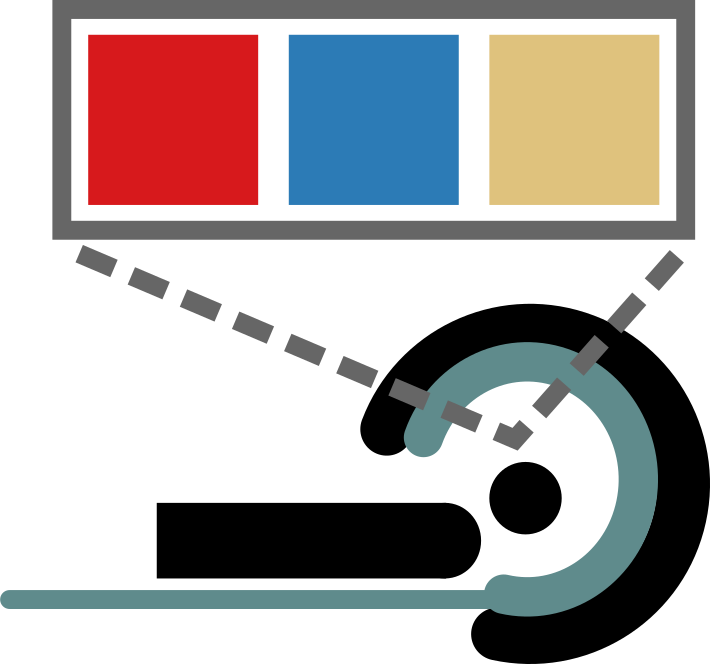
\includegraphics[scale=0.25]{figures/scanner_task.png}
    \end{center}

    This means that during scanning, the participant performs a behavioral task.

\end{frame}
\begin{frame}
    \frametitle{fMRI data}

    Structural MRI images are 3-D. fMRI adds a new dimension: time. That
    allows us to analyse how brain activity changes during the task.

    \begin{center}
        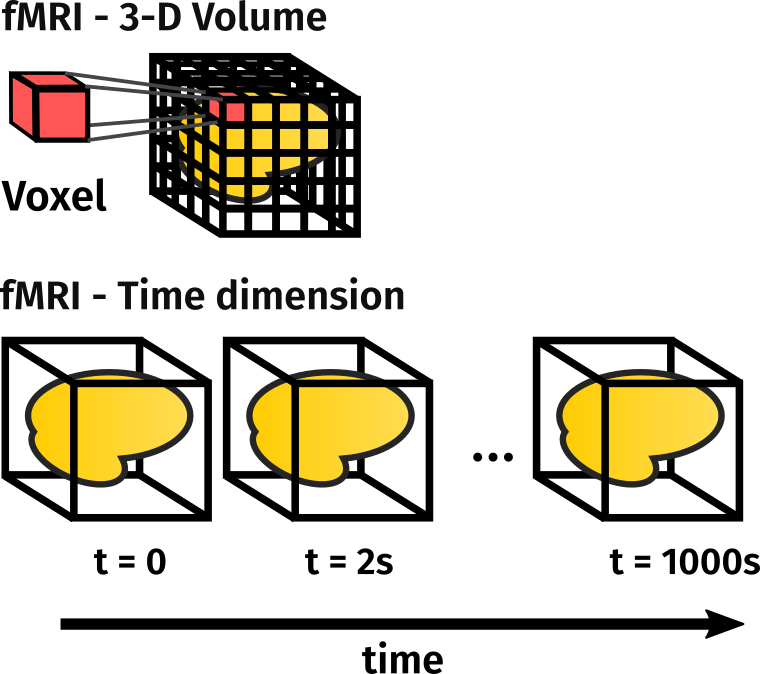
\includegraphics[scale=0.25]{figures/4d_data.png}
    \end{center}

    A typical fMRI session consists of around $10^2$ 3-D volumes, and each 3-D
    volume contains $10^5$ to $10^6$ voxels.

\end{frame}
\begin{frame}
    \frametitle{Putting it all together}
    
    We can analyse the data to detect changes in activation using a General
    Linear Model (GLM), a massive-univariate analysis.

    \begin{center}
        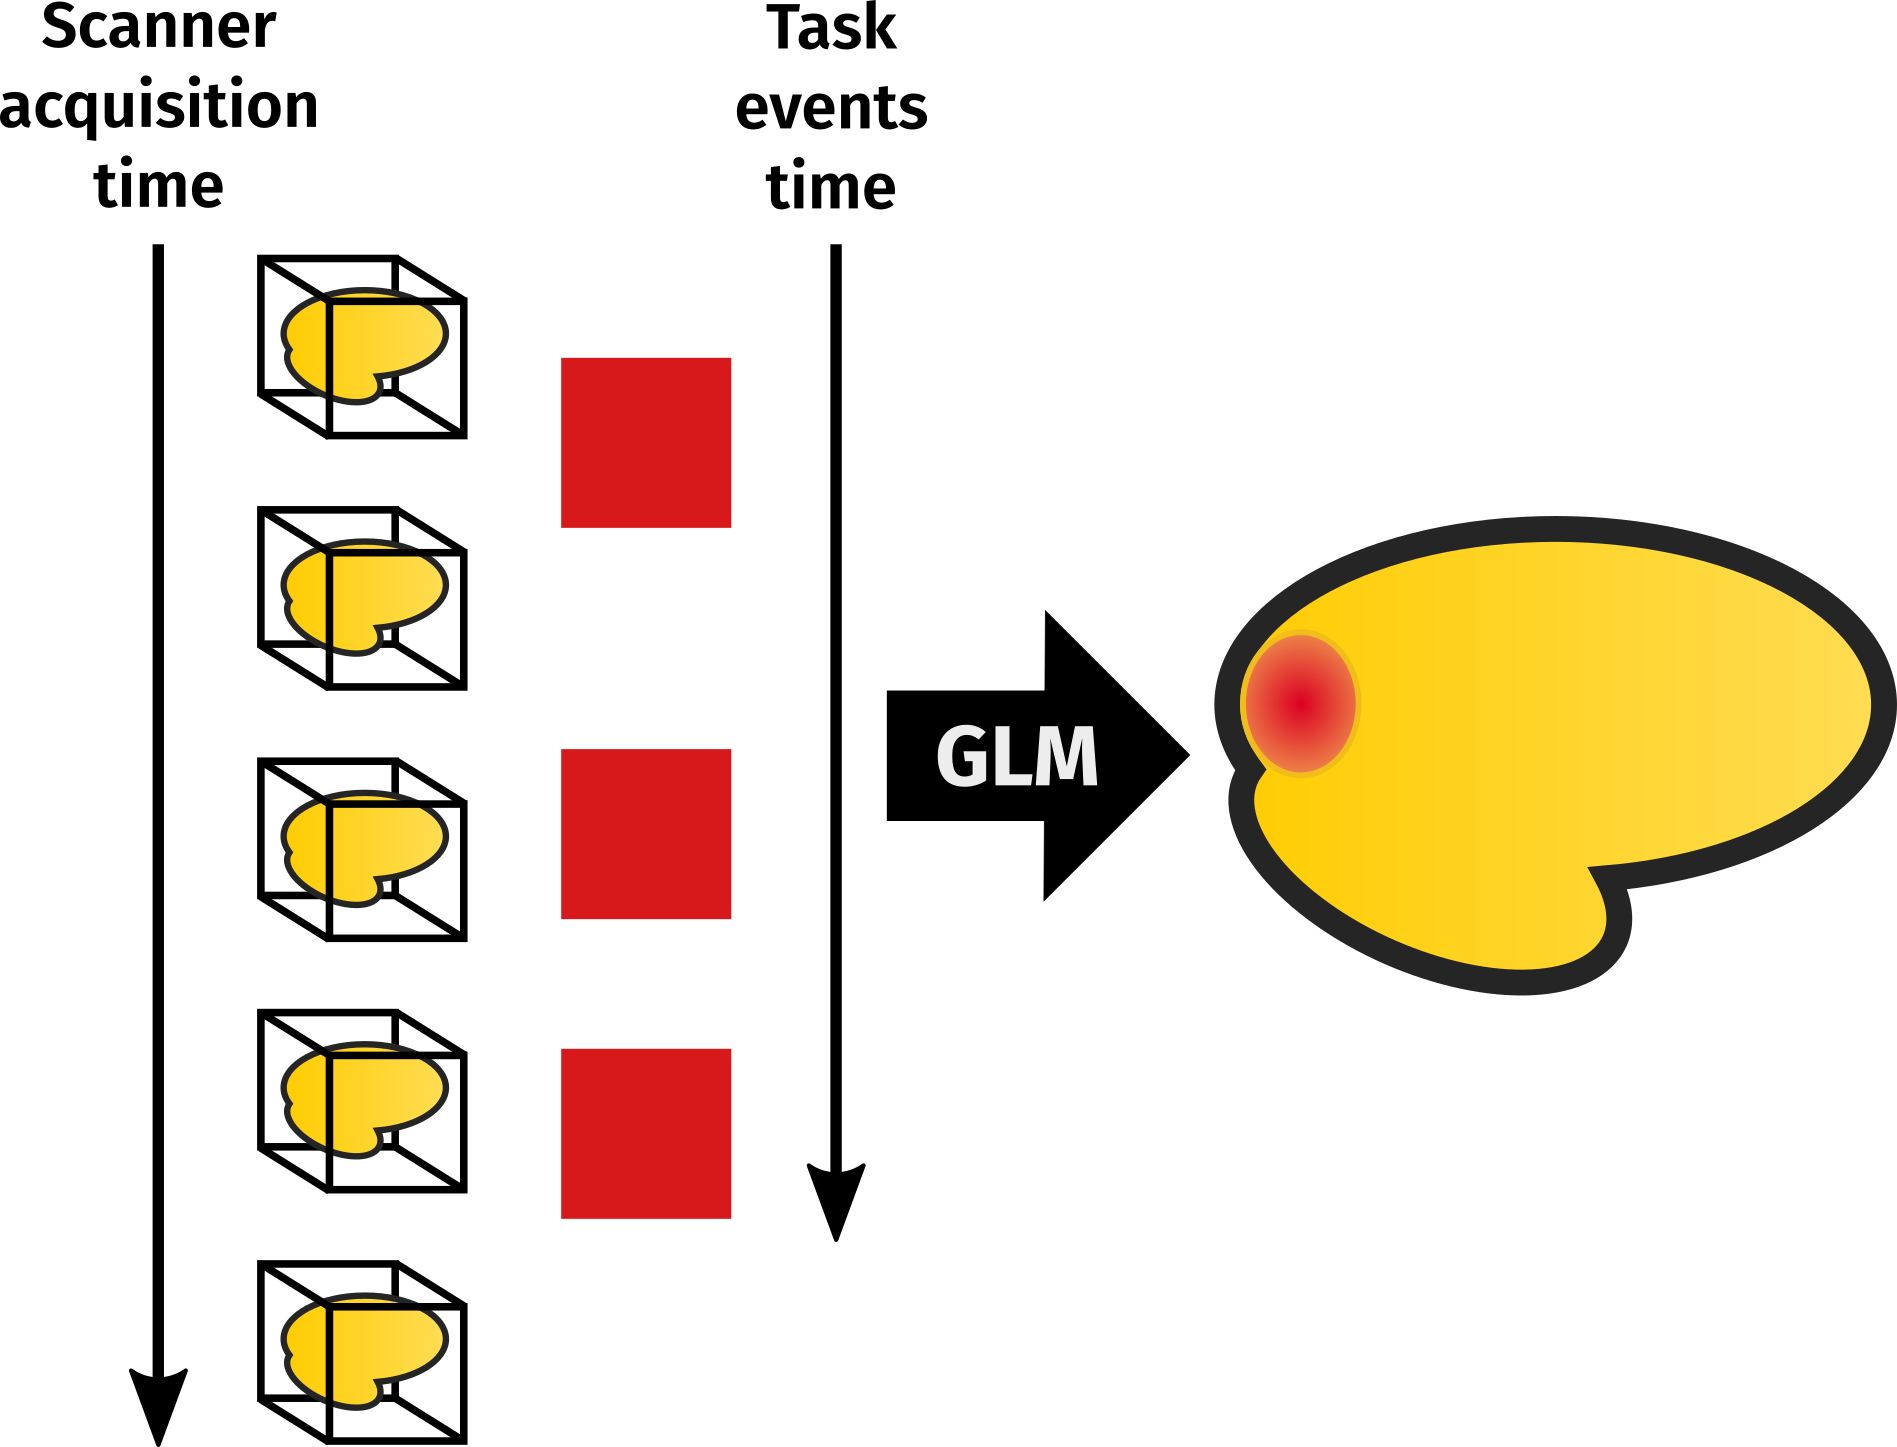
\includegraphics[scale=0.15]{figures/glm.png}
    \end{center}

\end{frame}

\section{Decoding}
\label{sec:Decoding}

\begin{frame}
    \frametitle{Asking about categories}

    Maybe we would like to ask different scientific questions:
    \begin{enumerate}
        \item Can we distinguish categories from the task?
        \item Can we find the voxels that discriminate among those categories?
    \end{enumerate}

    \begin{center}
        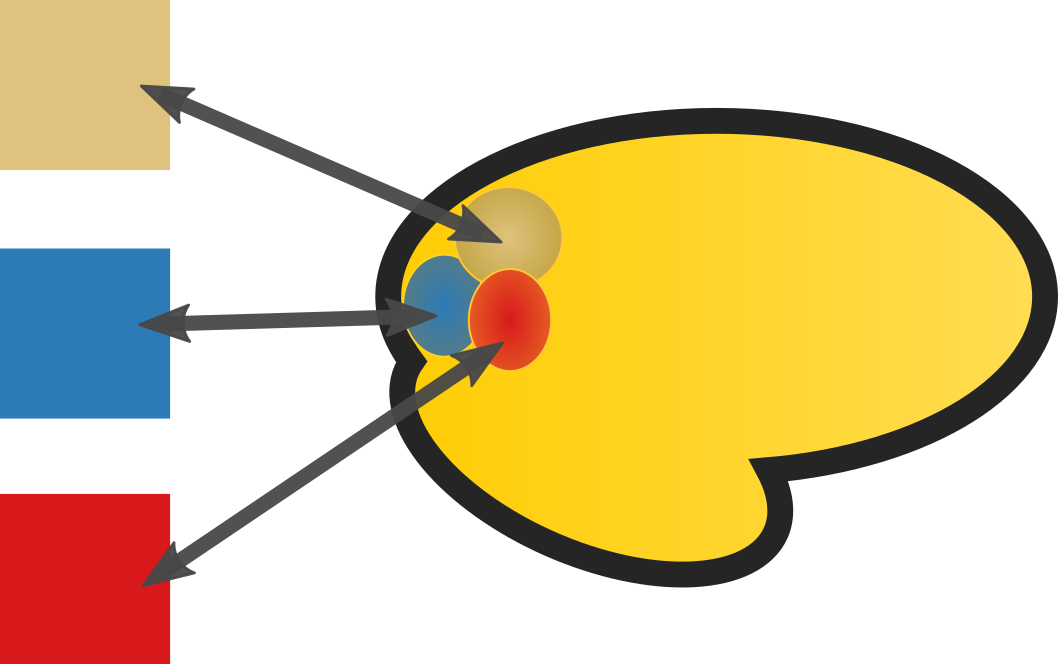
\includegraphics[scale=0.2]{figures/decoding.png}
    \end{center}

\end{frame}

\begin{frame}
    \frametitle{Model}
    Our proposal to answer those questions is to use a linear model. We need
    some help, however. We have too many voxels (features) and too few images
    (samples). 

    \[y = Xw\]

    That is why we add an extra term to the problem to be solved called
    regularization, $J(w)$.

    \[\hat{w} = \argmin_{w} \mathcal{L}\left(y, X, w \right) + J(w) \]

    The solution that we obtain is a vector of weights, $\hat{w}$. One weight
    per voxel.
\end{frame}

\begin{frame}{If things were this easy\ldots}
    Only two features (e.g., voxels) and many samples:

    \begin{center}
        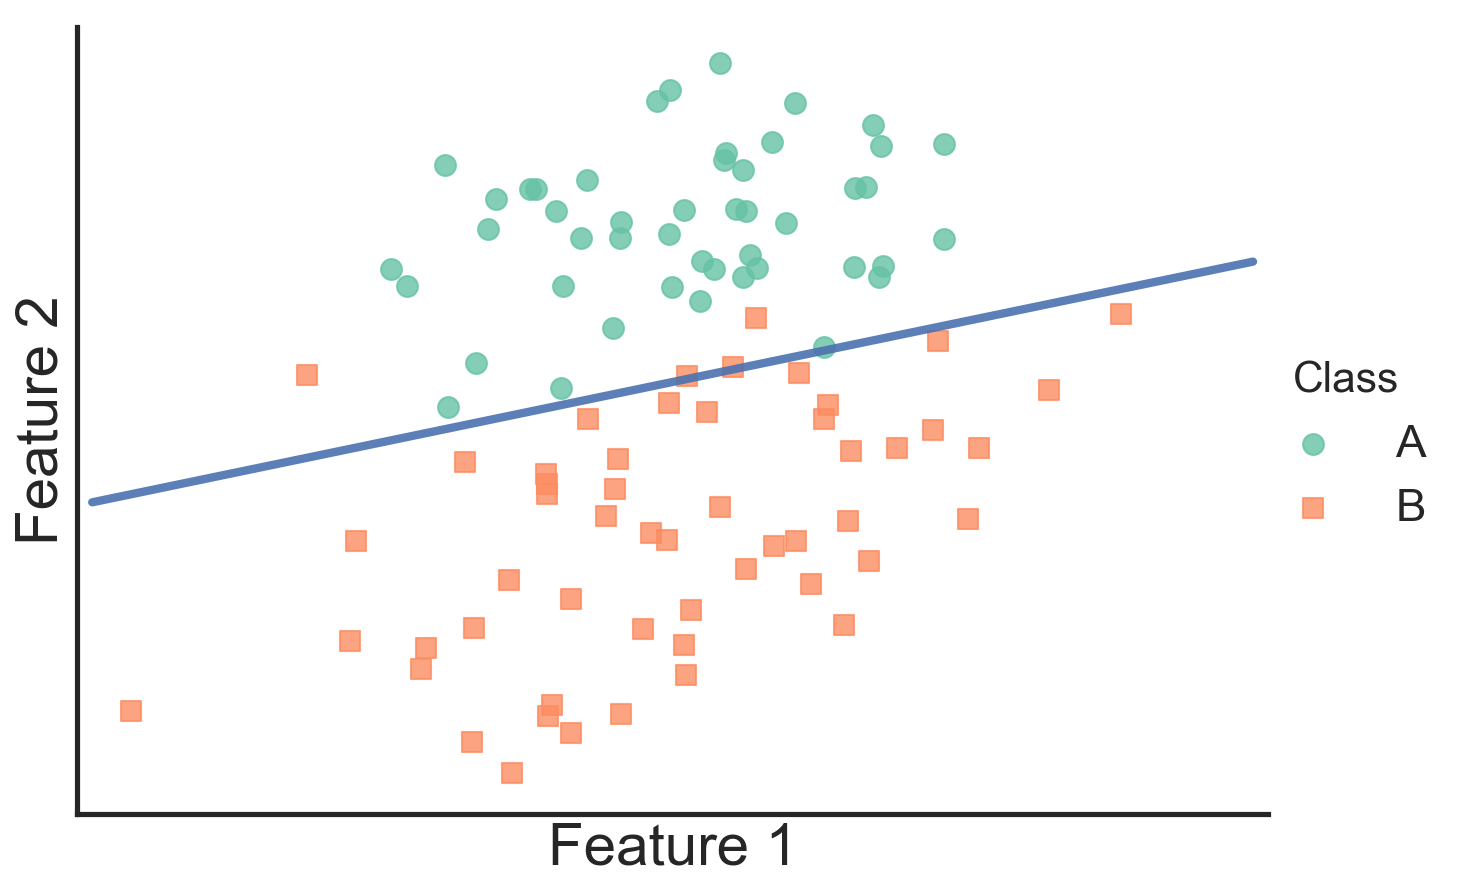
\includegraphics[scale=0.3]{figures/grad_descent_result.png}        
    \end{center}
\end{frame}

\begin{frame}{How does it look with real data?}

    In this task, participants could be in any of four different rooms. We ask
    the decoder if it can tell us in which room is the participant.

    \begin{center}
        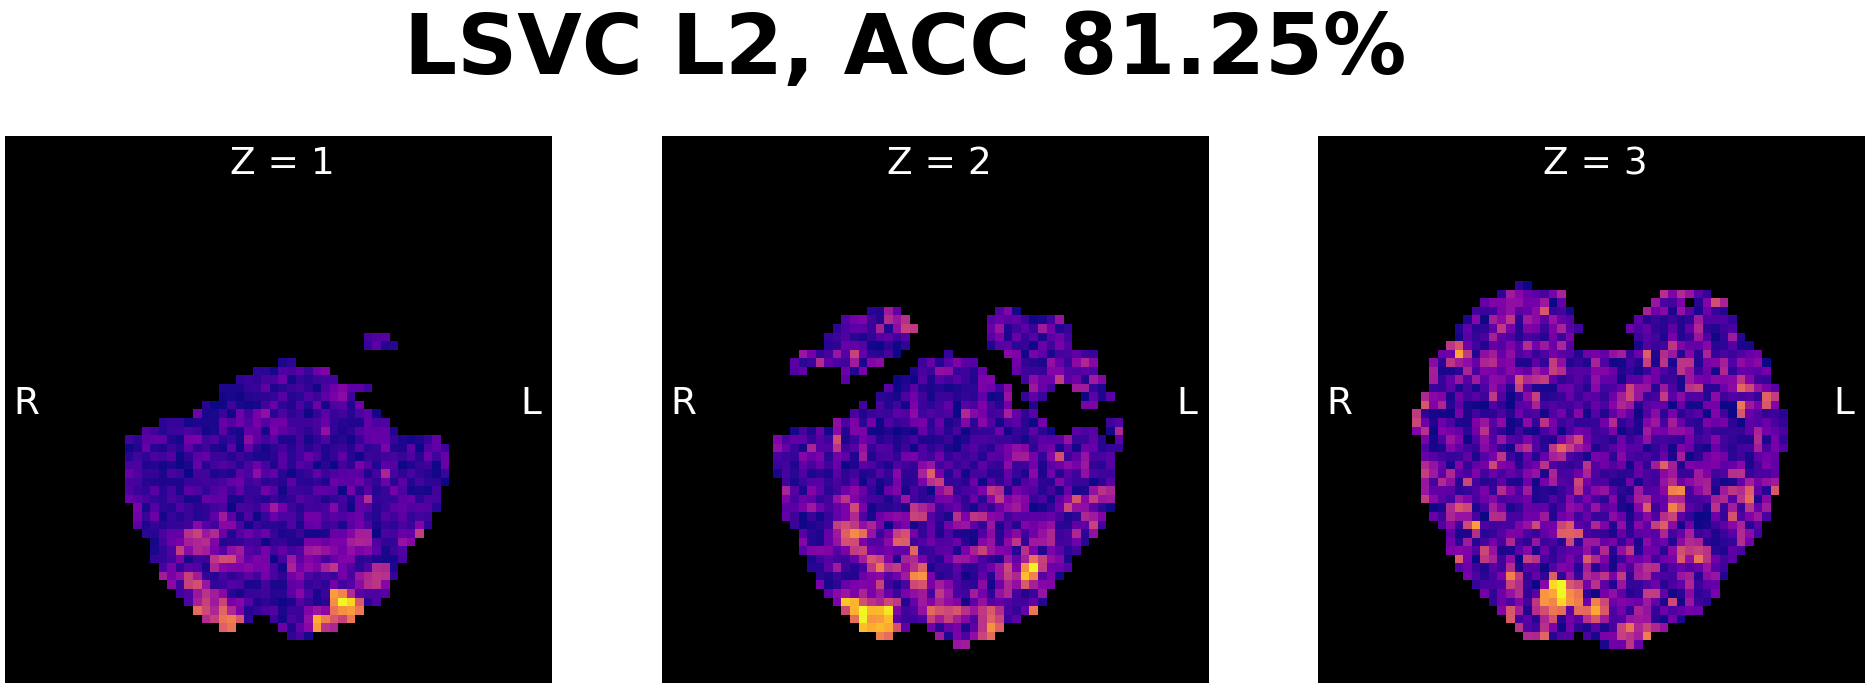
\includegraphics[scale=0.7]{figures/lsvc_l2-axial.png}
    \end{center}

    This is a \emph{dense} solution. It is easy to see where are the main areas
    involved, but what about the rest?

\end{frame}

\section{Structured sparsity}
\label{sec:Structured sparsity}

\begin{frame}
    \frametitle{Sparsity}
    The so-called LASSO or $l_1$ regularization impose \emph{sparsity} in the
    solution, i.e., non-informative features are weighted 0. 

    \begin{center}
        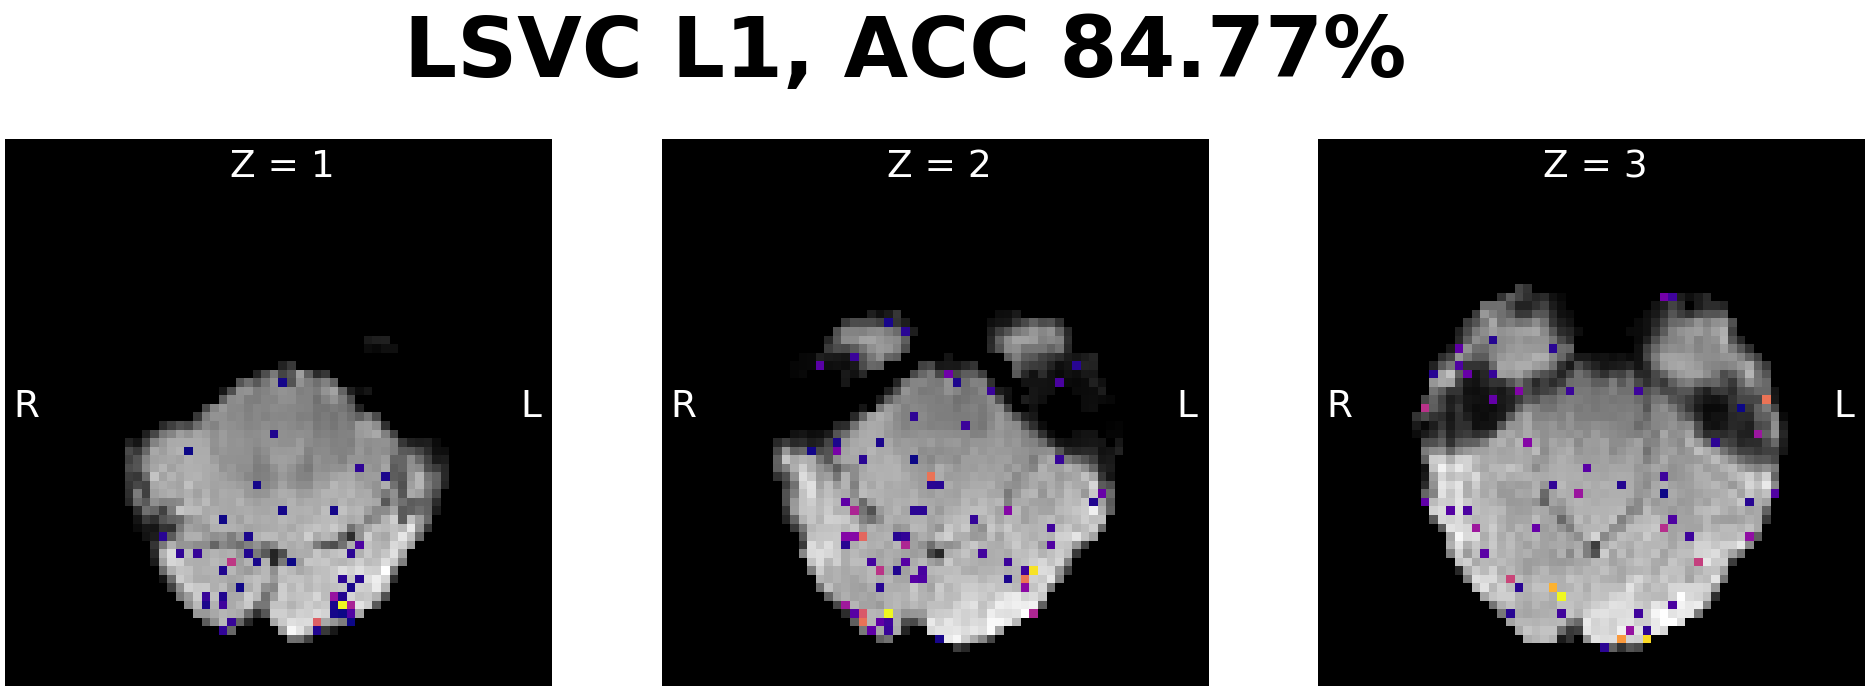
\includegraphics[scale=0.7]{figures/lsvc_l1-axial.png}
    \end{center}

    This makes the solution directly more interpretable, but are those voxels
    too few?  

\end{frame}
\begin{frame}
    \frametitle{Structured sparsity\footprnifullcite{baldassarre2012a}}
    We would like to reach a middle ground between a sparse and a dense
    solution where whole relevant areas involved in category discrimination are
    weighted different from 0.


\end{frame}
\begin{frame}
    \frametitle{BrainOwl}
    BrainOwl is a classifier based on the \emph{Ordered Weighted} $l_1$
    (OWL)\footlessfullcite{zeng2014-owl} norm.

    \[J_v(w) = \sum_{i=1}^{n} |w|_{[i]} v_i = v^T |w|_{\downarrow}\]

    There are Implementations of another interesting structured sparsity
    decoders implemented like \emph{Sparse Total Variation}
    (TV-$l_1$)\footprnifullcite{gramfort2013} or
    \emph{Graph-Net}\footlessfullcite{grosenick2013}.

\end{frame}
\begin{frame}
    \frametitle{The story so far}
    
    Dense, sparse, and structured sparse solutions from simulated data in
    manually segmented subiculum.

    \begin{center}
        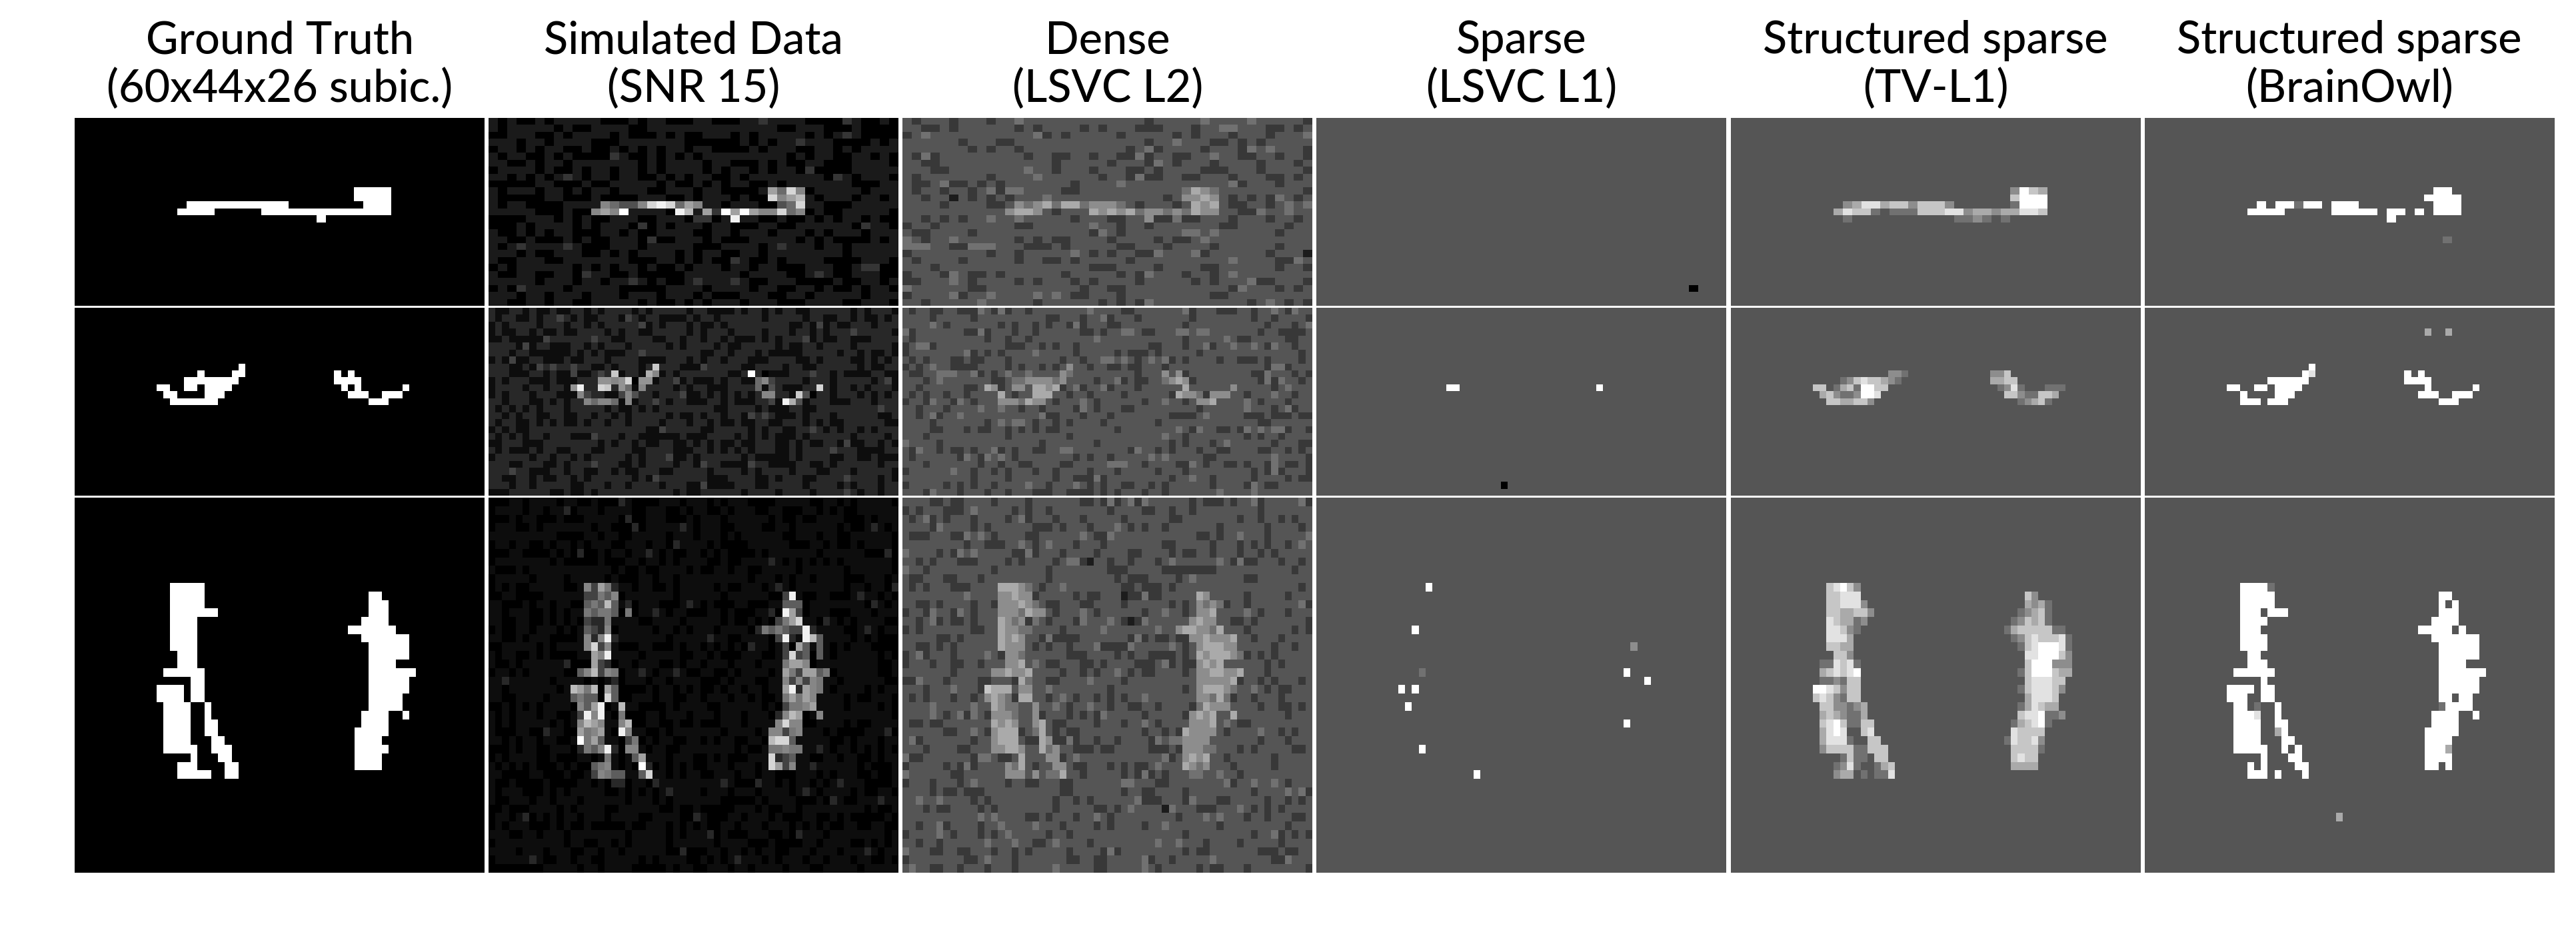
\includegraphics[scale=0.35]{figures/template_and_weights_4_clfs.png}
    \end{center}

\end{frame}
\begin{frame}
    \frametitle{Rooms question revisited}


    \begin{center}
        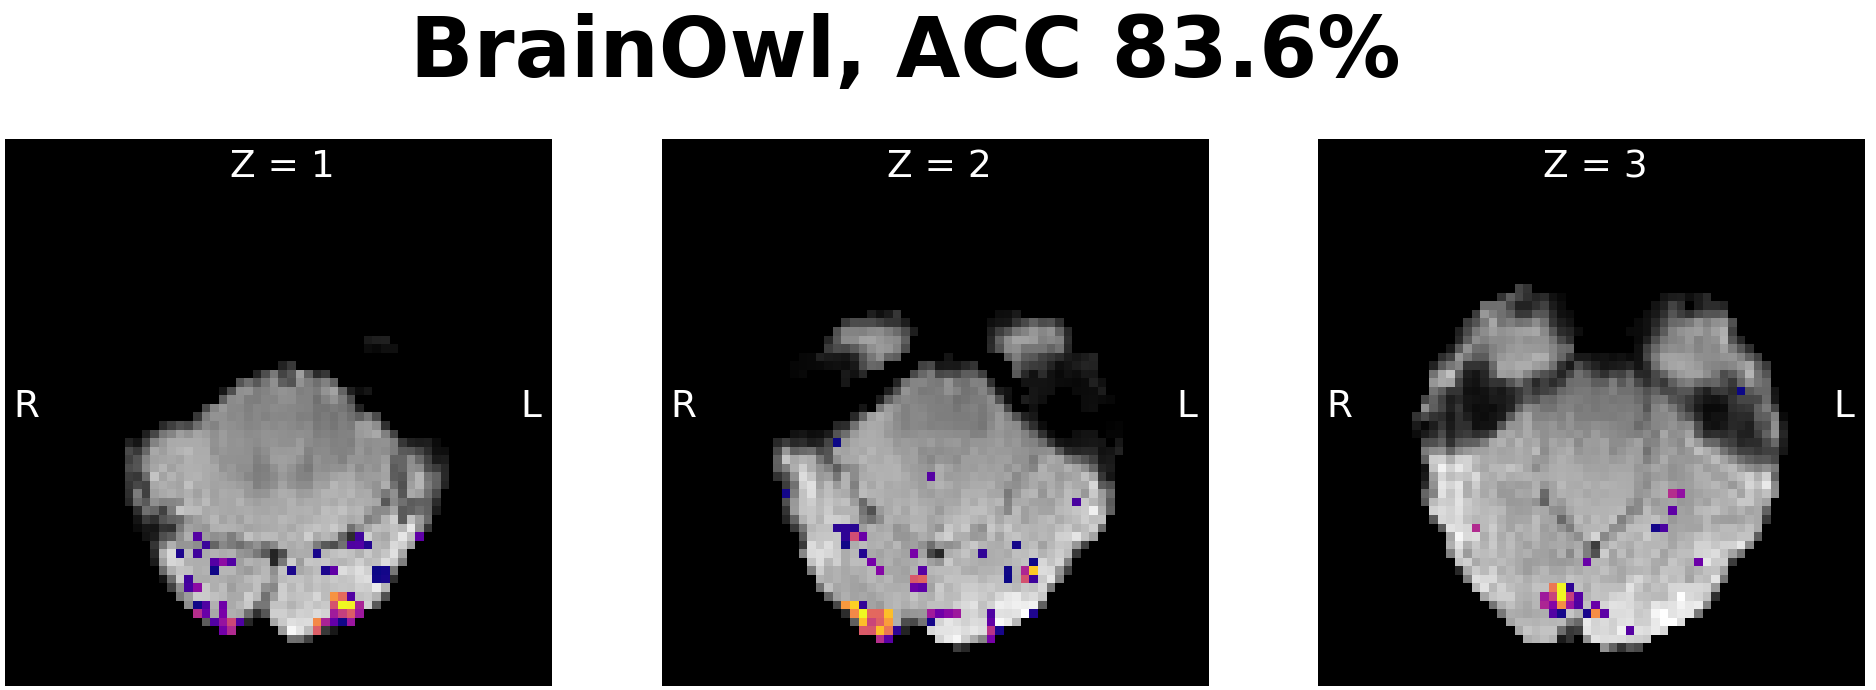
\includegraphics[scale=0.7]{figures/brainowl-axial.png}
    \end{center}
\end{frame}

% option [t] causes text to be flushed to the top
\begin{frame}[t]
  \frametitle{Why structured sparsity?}
  In a multivariate analysis,
  \begin{itemize}
  \item take into consideration spatial and temporal information,
  \item recover the \emph{true} activation maps,
  \item ease interpretation of results.
  \end{itemize}
    % \footlessfullcite{Grosenick2013} 
\end{frame}

\begin{frame}
  \frametitle{How is it implemented?}
  Structured sparsity
  \begin{itemize}
  \item can be implemented as a \textbf{regression} problem,
  \item that can be extended to \textbf{decoding},
  \item and incorporates structural and temporal priors as
    \textbf{regularization} terms.
  \end{itemize}
\end{frame}
\begin{frame}
  \frametitle{Regression}
  \begin{columns}
    \begin{column}{0.55\linewidth}
      A regression problem as a linear model is well known 
      \[\mathbf{y} = f(\mathbf{X}, \mathbf{y}) = F(\mathbf{Xw}) = \mathbf{Xw}\]
      % and has a closed-form solution
      % \[\mathbf{X}^{T}\left( \mathbf{y} - \mathbf{Xw} \right) = 0\]
      and can be solved as an optimization problem to find the \emph{normal equations}
      \[\hat{\mathbf{w}} = \left( \mathbf{X}^{T}\mathbf{X}\right)^{-1}\mathbf{X}^{T}\mathbf{y}\]
    \end{column}
    \begin{column}{0.45\linewidth}
      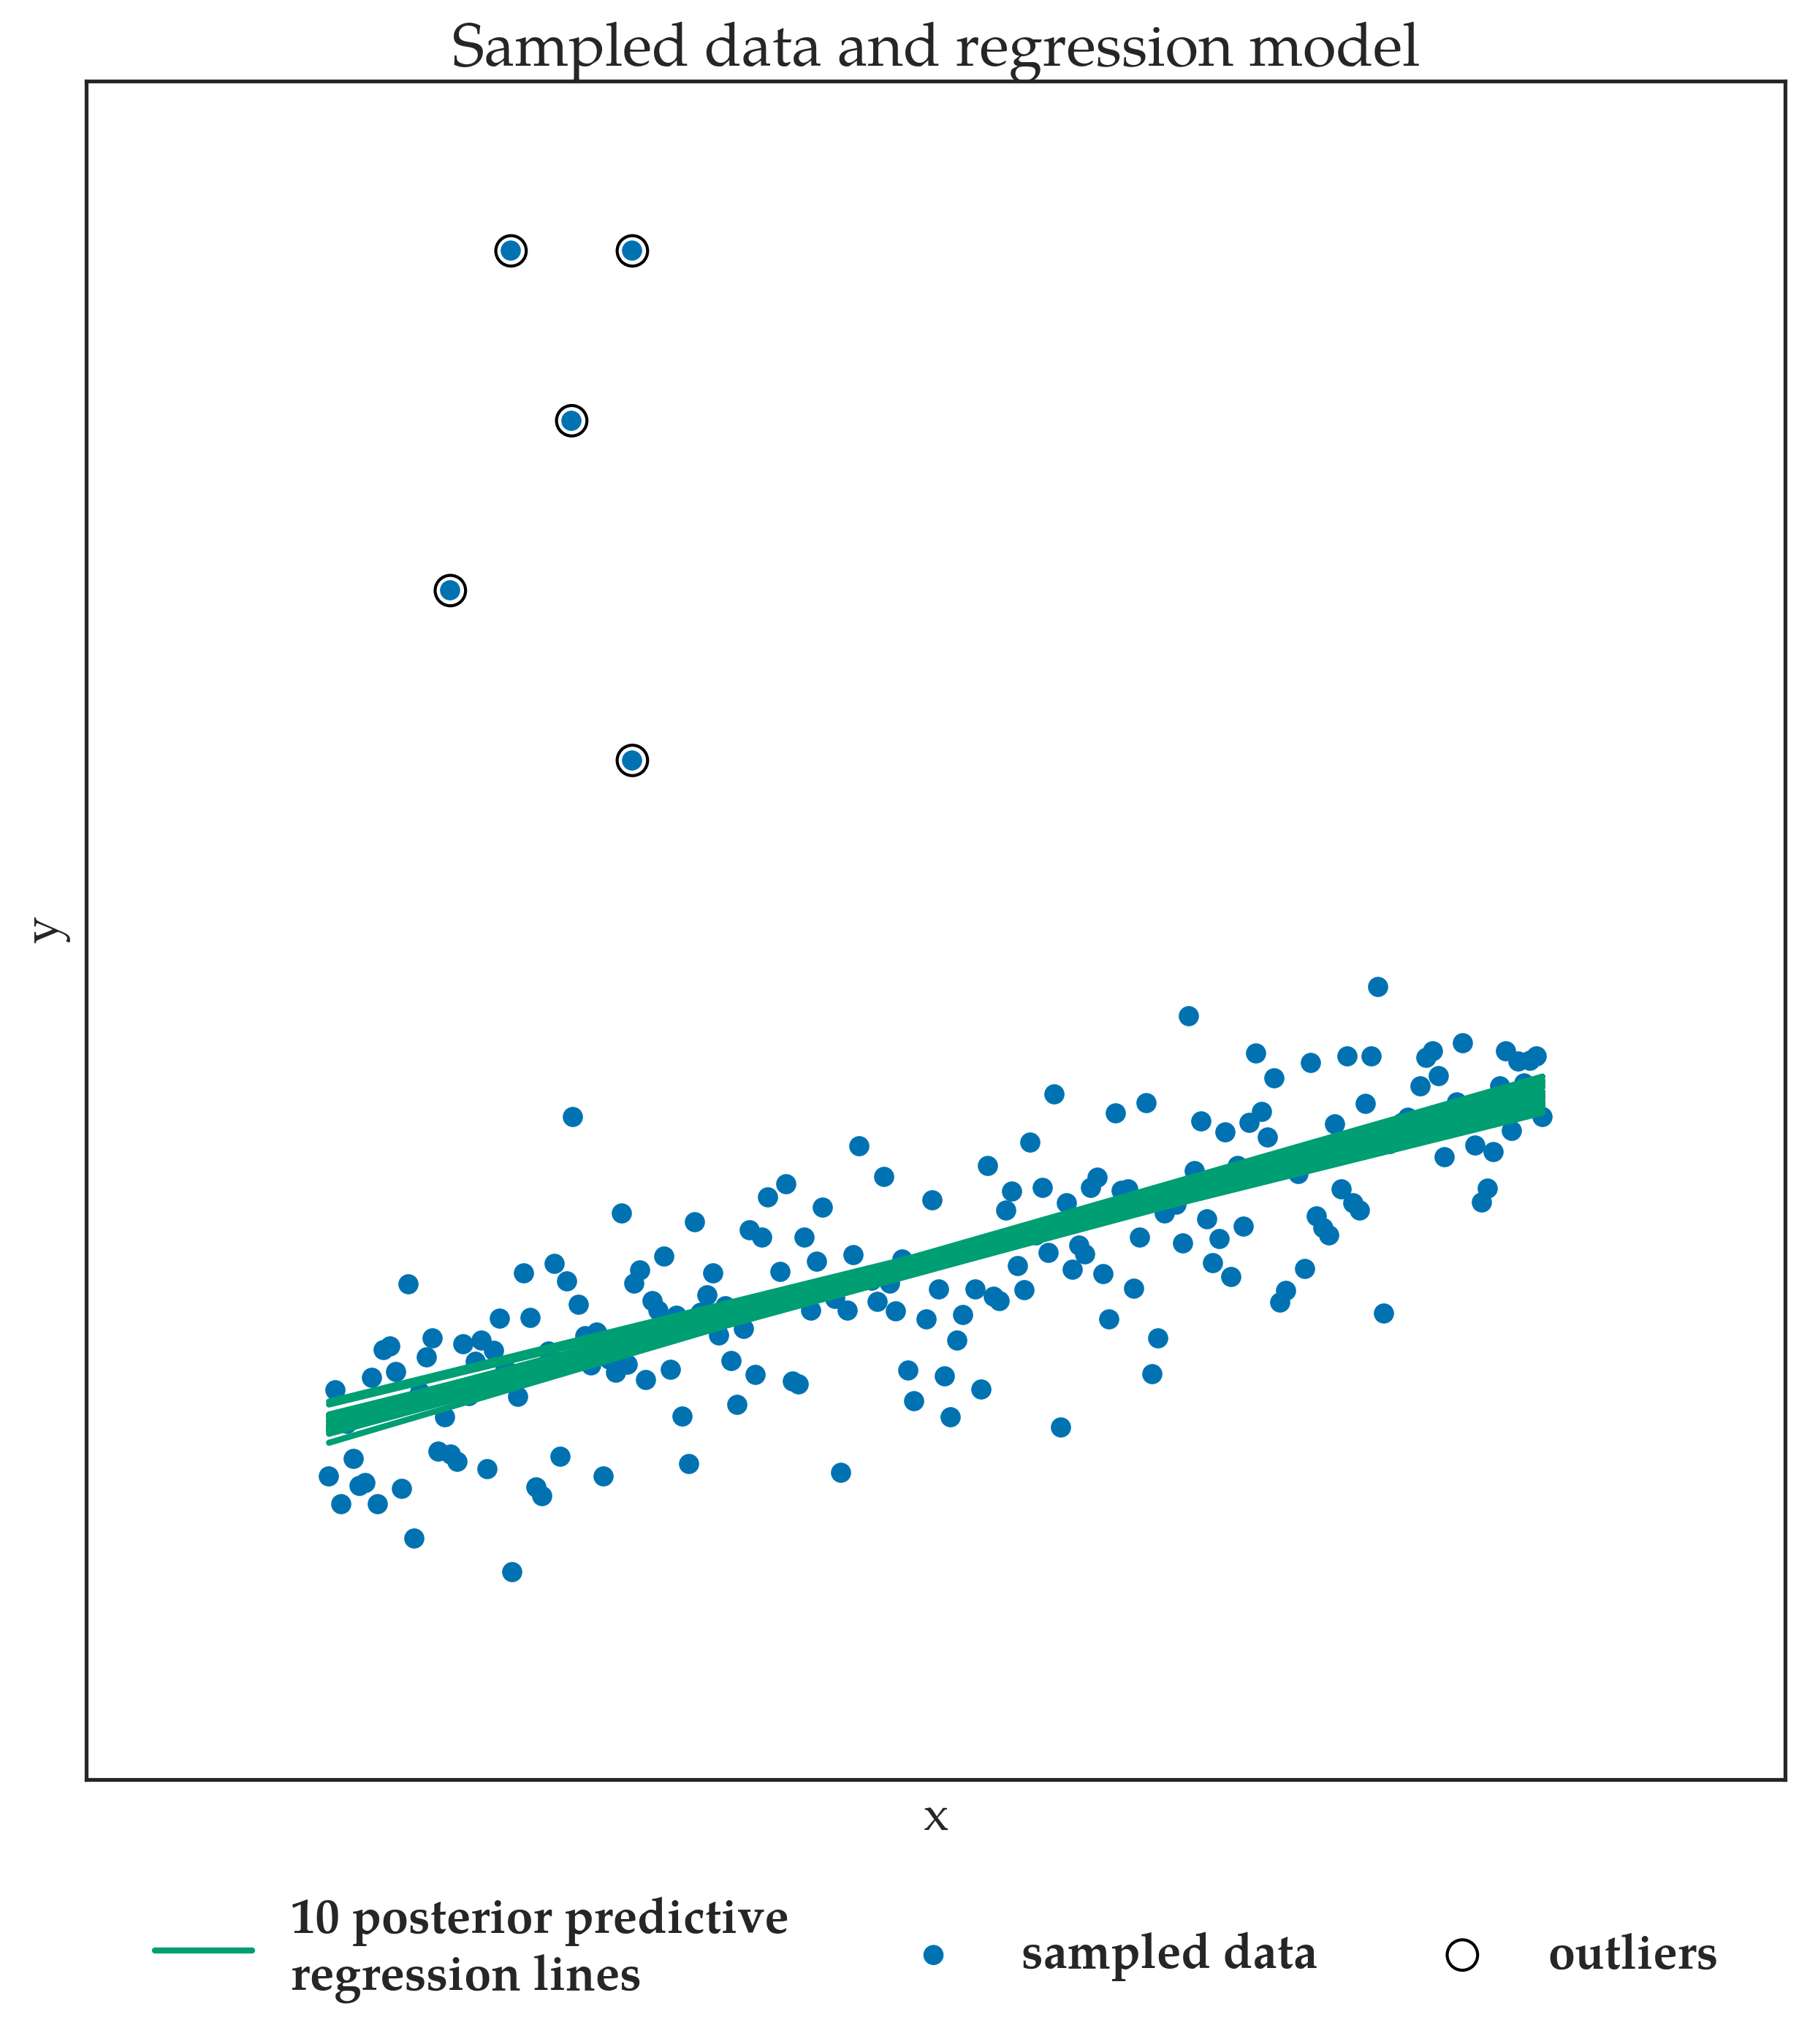
\includegraphics[scale=0.25]{figures/robust_linear_regression_with_outliers.png}
    \end{column}
  \end{columns}
  % \vspace{0.5cm}
\end{frame}
\begin{frame}[t]
  \frametitle{Regression and Polynomials}
  \begin{columns}
    \begin{column}{1.1\textwidth}
      We are not restricted to linear relationships between \(\mathbf{X}\) and
      \(\mathbf{y}\), but careful with underfitting or overfitting: keep a
      validation set to test the model.
    \end{column}
  \end{columns}
  \begin{center}
    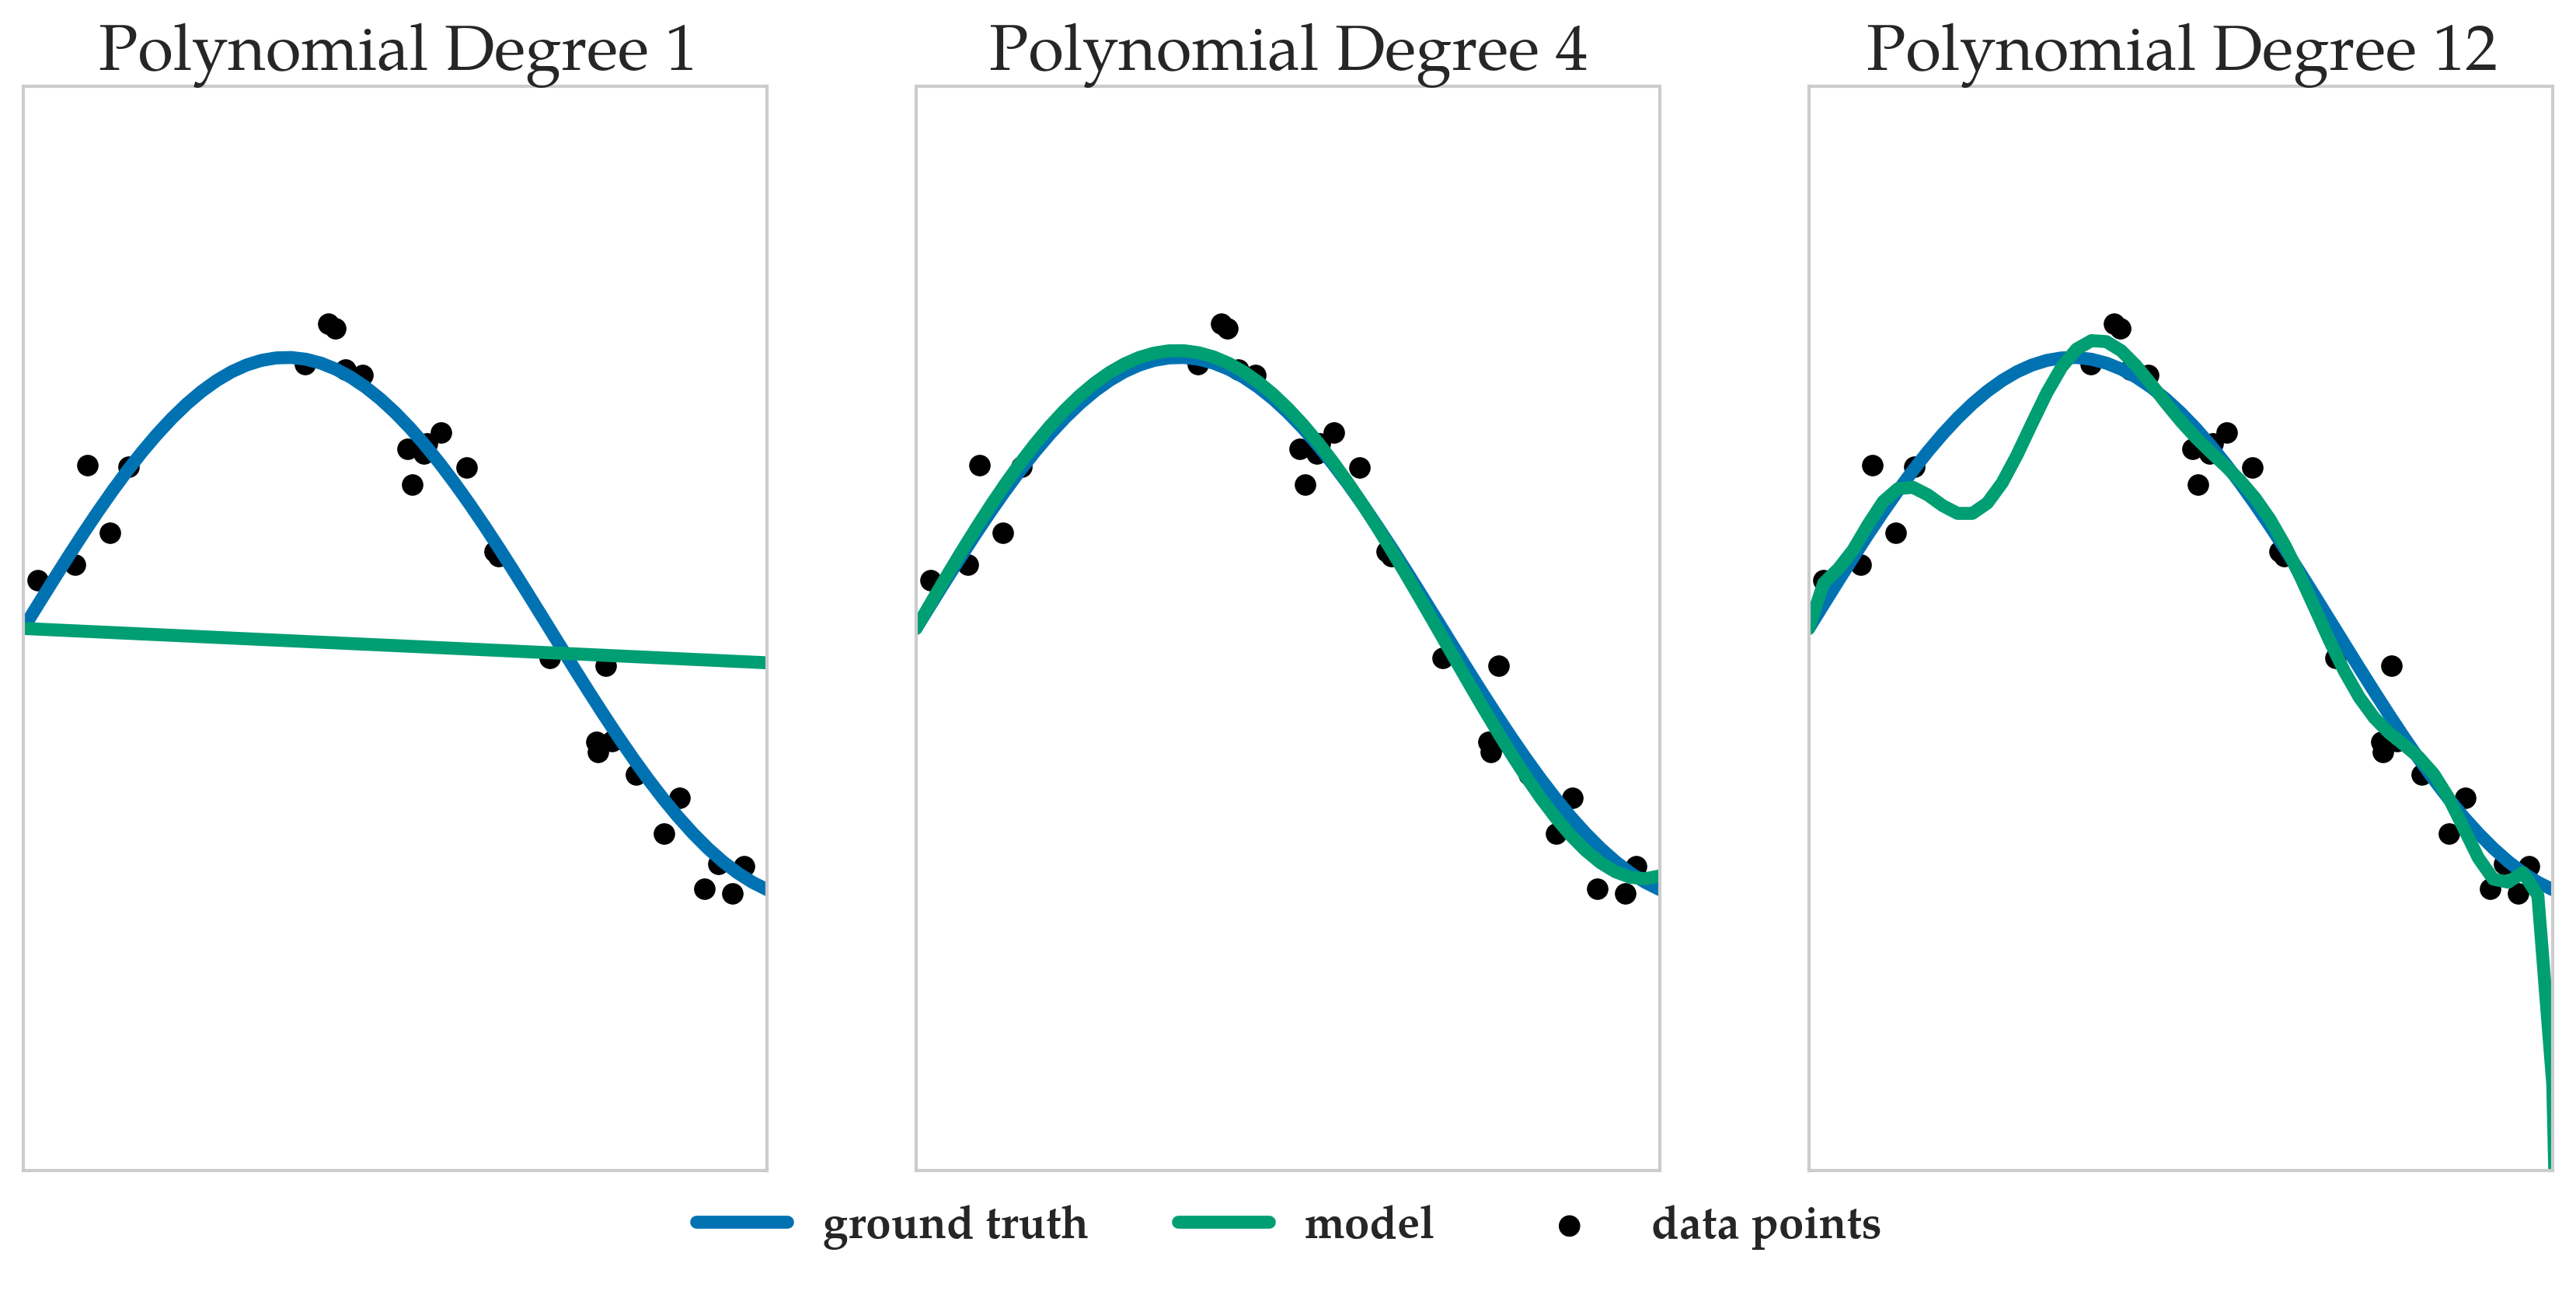
\includegraphics[scale=0.36]{figures/linear_model_underf_overf.png}
  \end{center}
  \begin{columns}
    \begin{column}{1.1\textwidth}
      For a discrete target variable, we have a classification problem; e.g.
      \(\mathrm{sign}\left(\mathbf{Xw}\right)\) where $\mathbf{y}$ is either $1$
      or $-1$.
    \end{column}
  \end{columns}
\end{frame}
\begin{frame}
  \frametitle{Classification: Interpretation}
  Depending on the classification problem, classifier accuracy might be
  misleading. 
  \begin{center}
    \includegraphics<1>[scale=0.22]{figures/moons_circles_linear_clf_1.png}
    \includegraphics<2>[scale=0.22]{figures/moons_circles_linear_clf_2.png}
    \includegraphics<3>[scale=0.22]{figures/moons_circles_linear_clf.png}
  \end{center}
\end{frame}
\begin{frame}
  \frametitle{Classification: Interpretation}
  A non-separable dataset in 1-D needs a non-linear transformation. 
  \begin{center}
    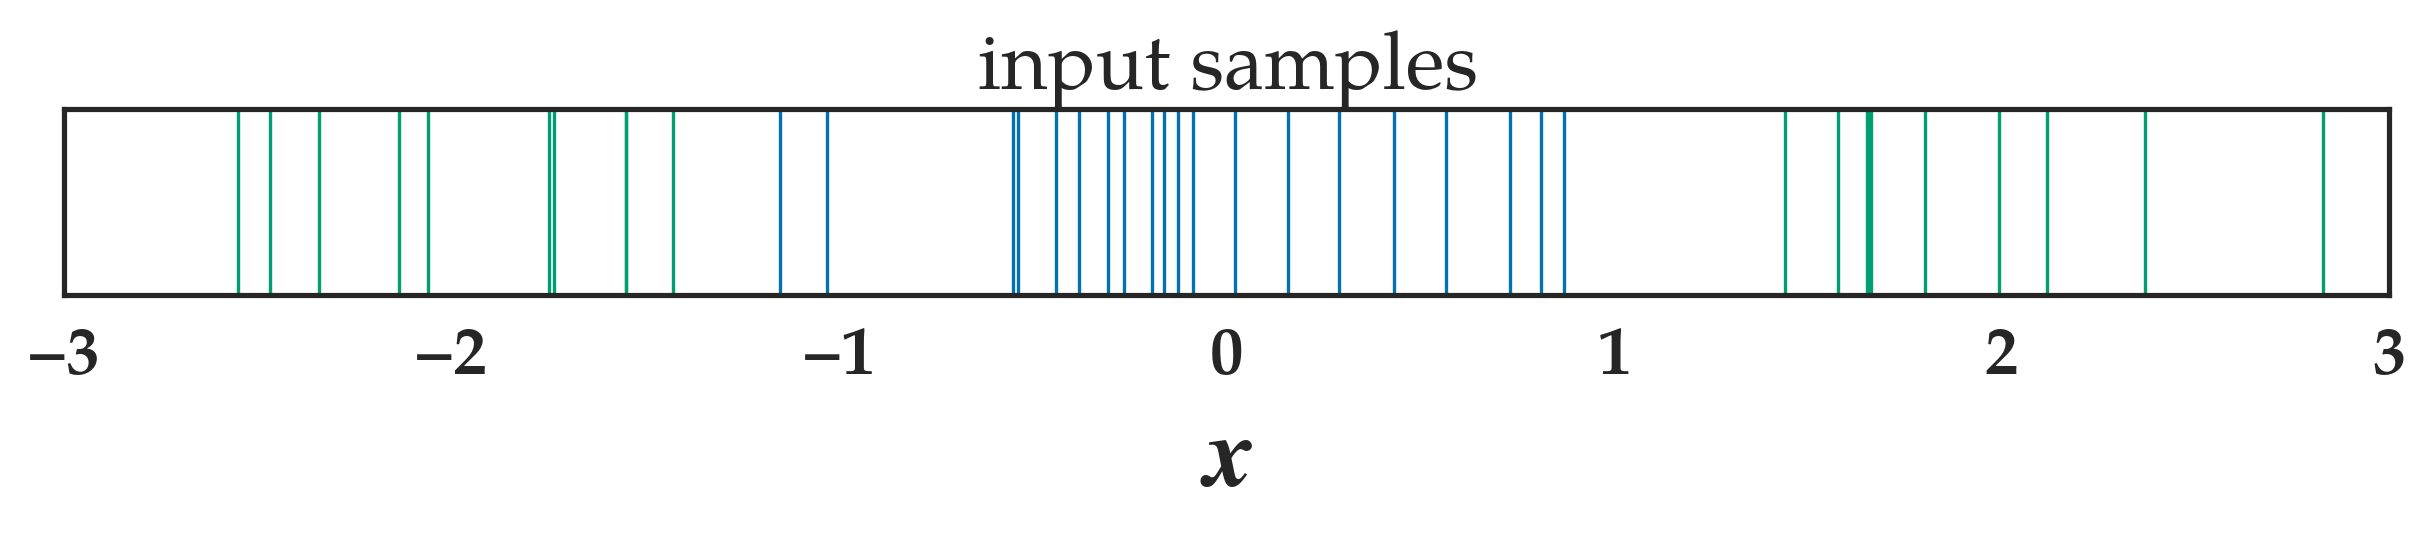
\includegraphics[scale=0.3]{figures/input_features.png}
  \end{center}
  \begin{center}
    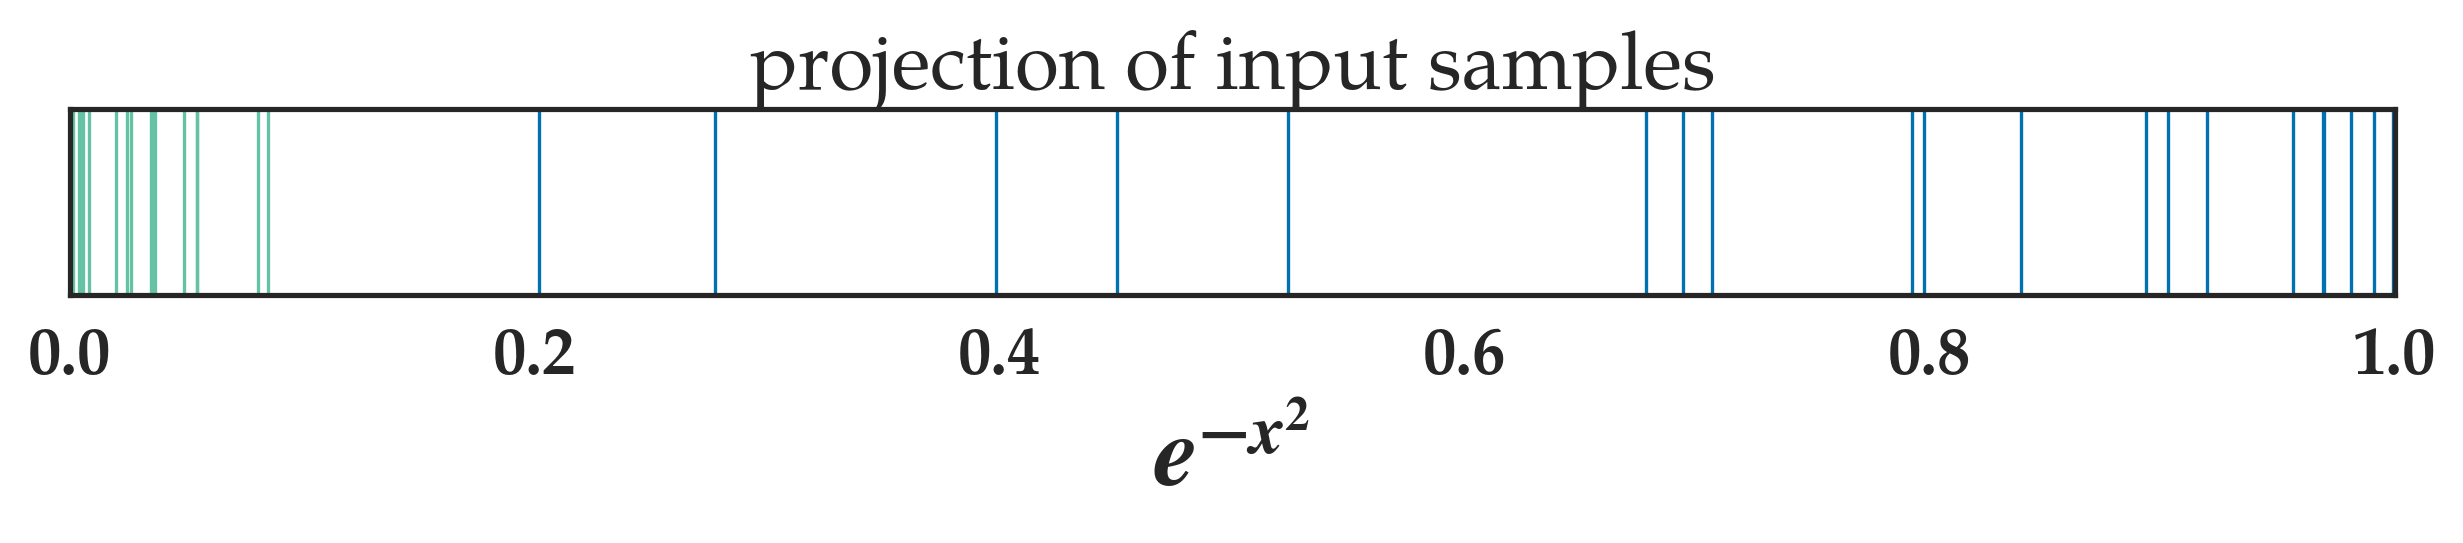
\includegraphics[scale=0.3]{figures/projection.png}
  \end{center}
  \begin{center}
    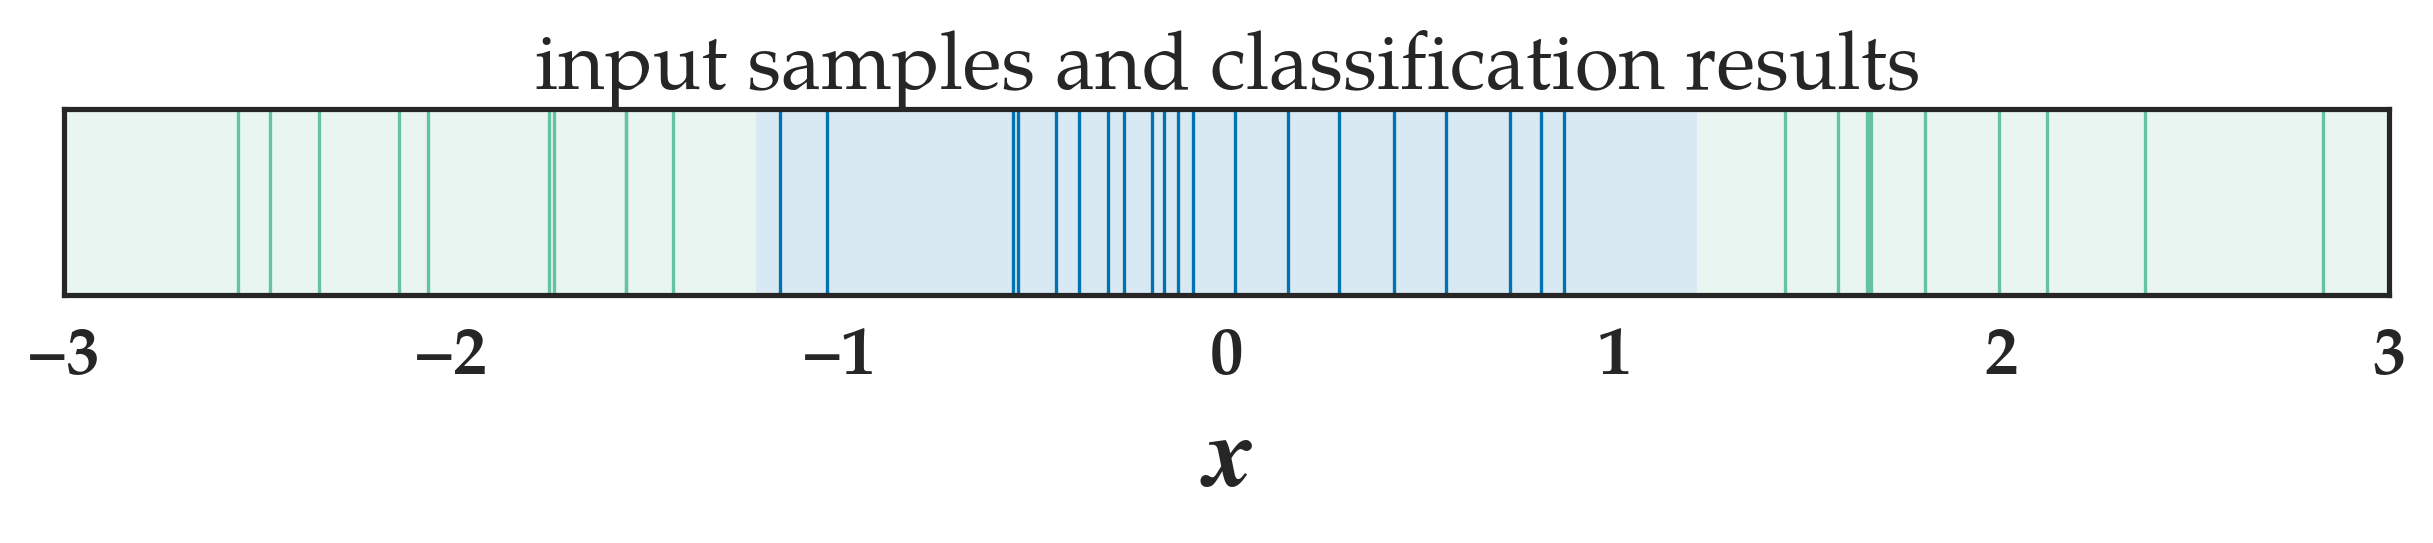
\includegraphics[scale=0.3]{figures/prediction.png}
  \end{center}
  After a projection the data can be linearly separated but back in the original space we have
  \emph{two} boundaries instead of one.
\end{frame}
\begin{frame}
  \frametitle{Regularization: Purpose}
  Regularization
  \begin{itemize}
  \item helps with overfitting,
  \item can do feature selection ($\rightarrow$ sparsity),
  \item and is necessary to solve the mathematical problem when the number of
    dimensions is very high (because it is ill-posed).
  \end{itemize}
  Regularization will also connect the ideas of structured and sparse
  solutions, together with a linear model.
\end{frame}
\begin{frame}
  \frametitle{Regularization: How does it do it?}
  Regularization is a term, \(J(\mathbf{w})\), added to the optimization problem:
  % \[\mathbf{y} = \mathbf{Xw} + \lambda{}J(\mathbf{w})\]
  \[\hat{\mathbf{w}} = \argmin_{\mathbf{w}} \lVert \mathbf{y} - \mathbf{Xw}
    \rVert^{2}_{2} + \lambda{}J(\mathbf{w})\]
  \begin{center}
    \begin{tabular}[h]{@{}lll@{}}
      & \(J(\mathbf{w})\) & Effect \\
      \cmidrule(r){2-3}
      Ridge, \(l_{2}\) & \(\lVert{\mathbf{w}}\rVert{}^{2}_{2} = \sum_{i=1}^{N}w_{i}^{2}\) & Shrinkage \\
      Lasso, \(l_{1}\) & \(\lVert{\mathbf{w}}\rVert_{1} = \sum_{i=1}^{N}\left| w_{i} \right|\) & Sparsity \\
    \end{tabular}
  \end{center}
  \begin{center}
    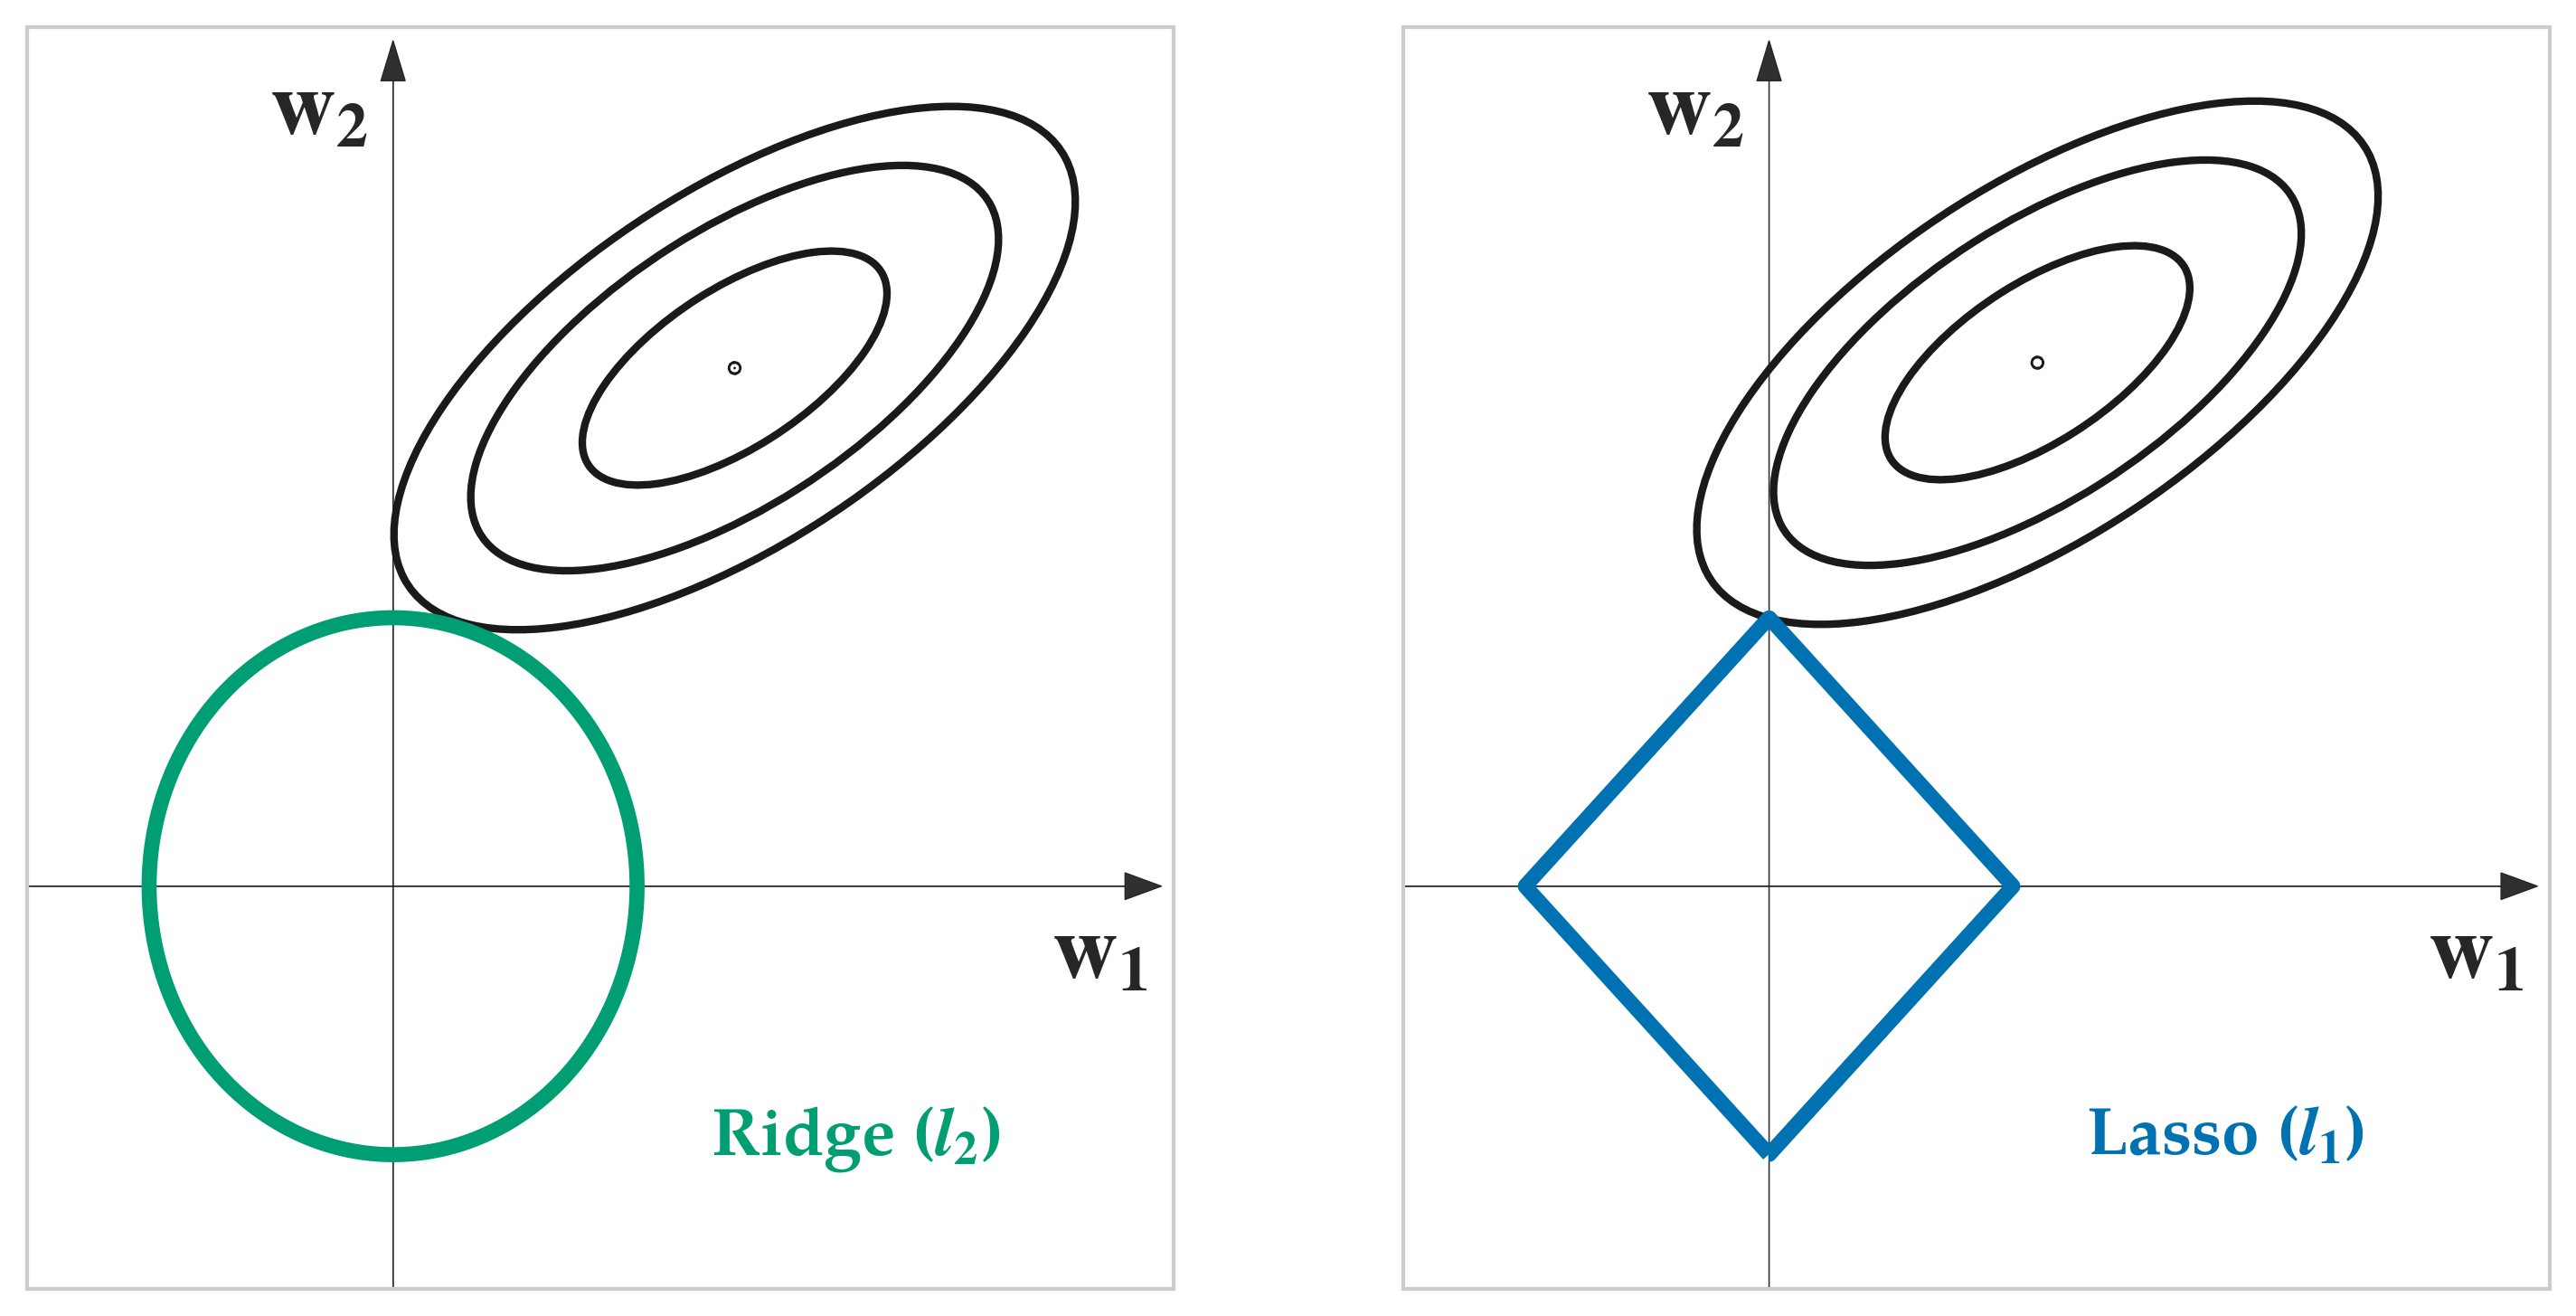
\includegraphics[scale=0.25]{figures/l1_l2_geometry.png}
  \end{center}
\end{frame}
\begin{frame}
  \frametitle{Regularization: Effect on Coefficients}
  \begin{columns}
    \begin{column}{0.5\linewidth}
      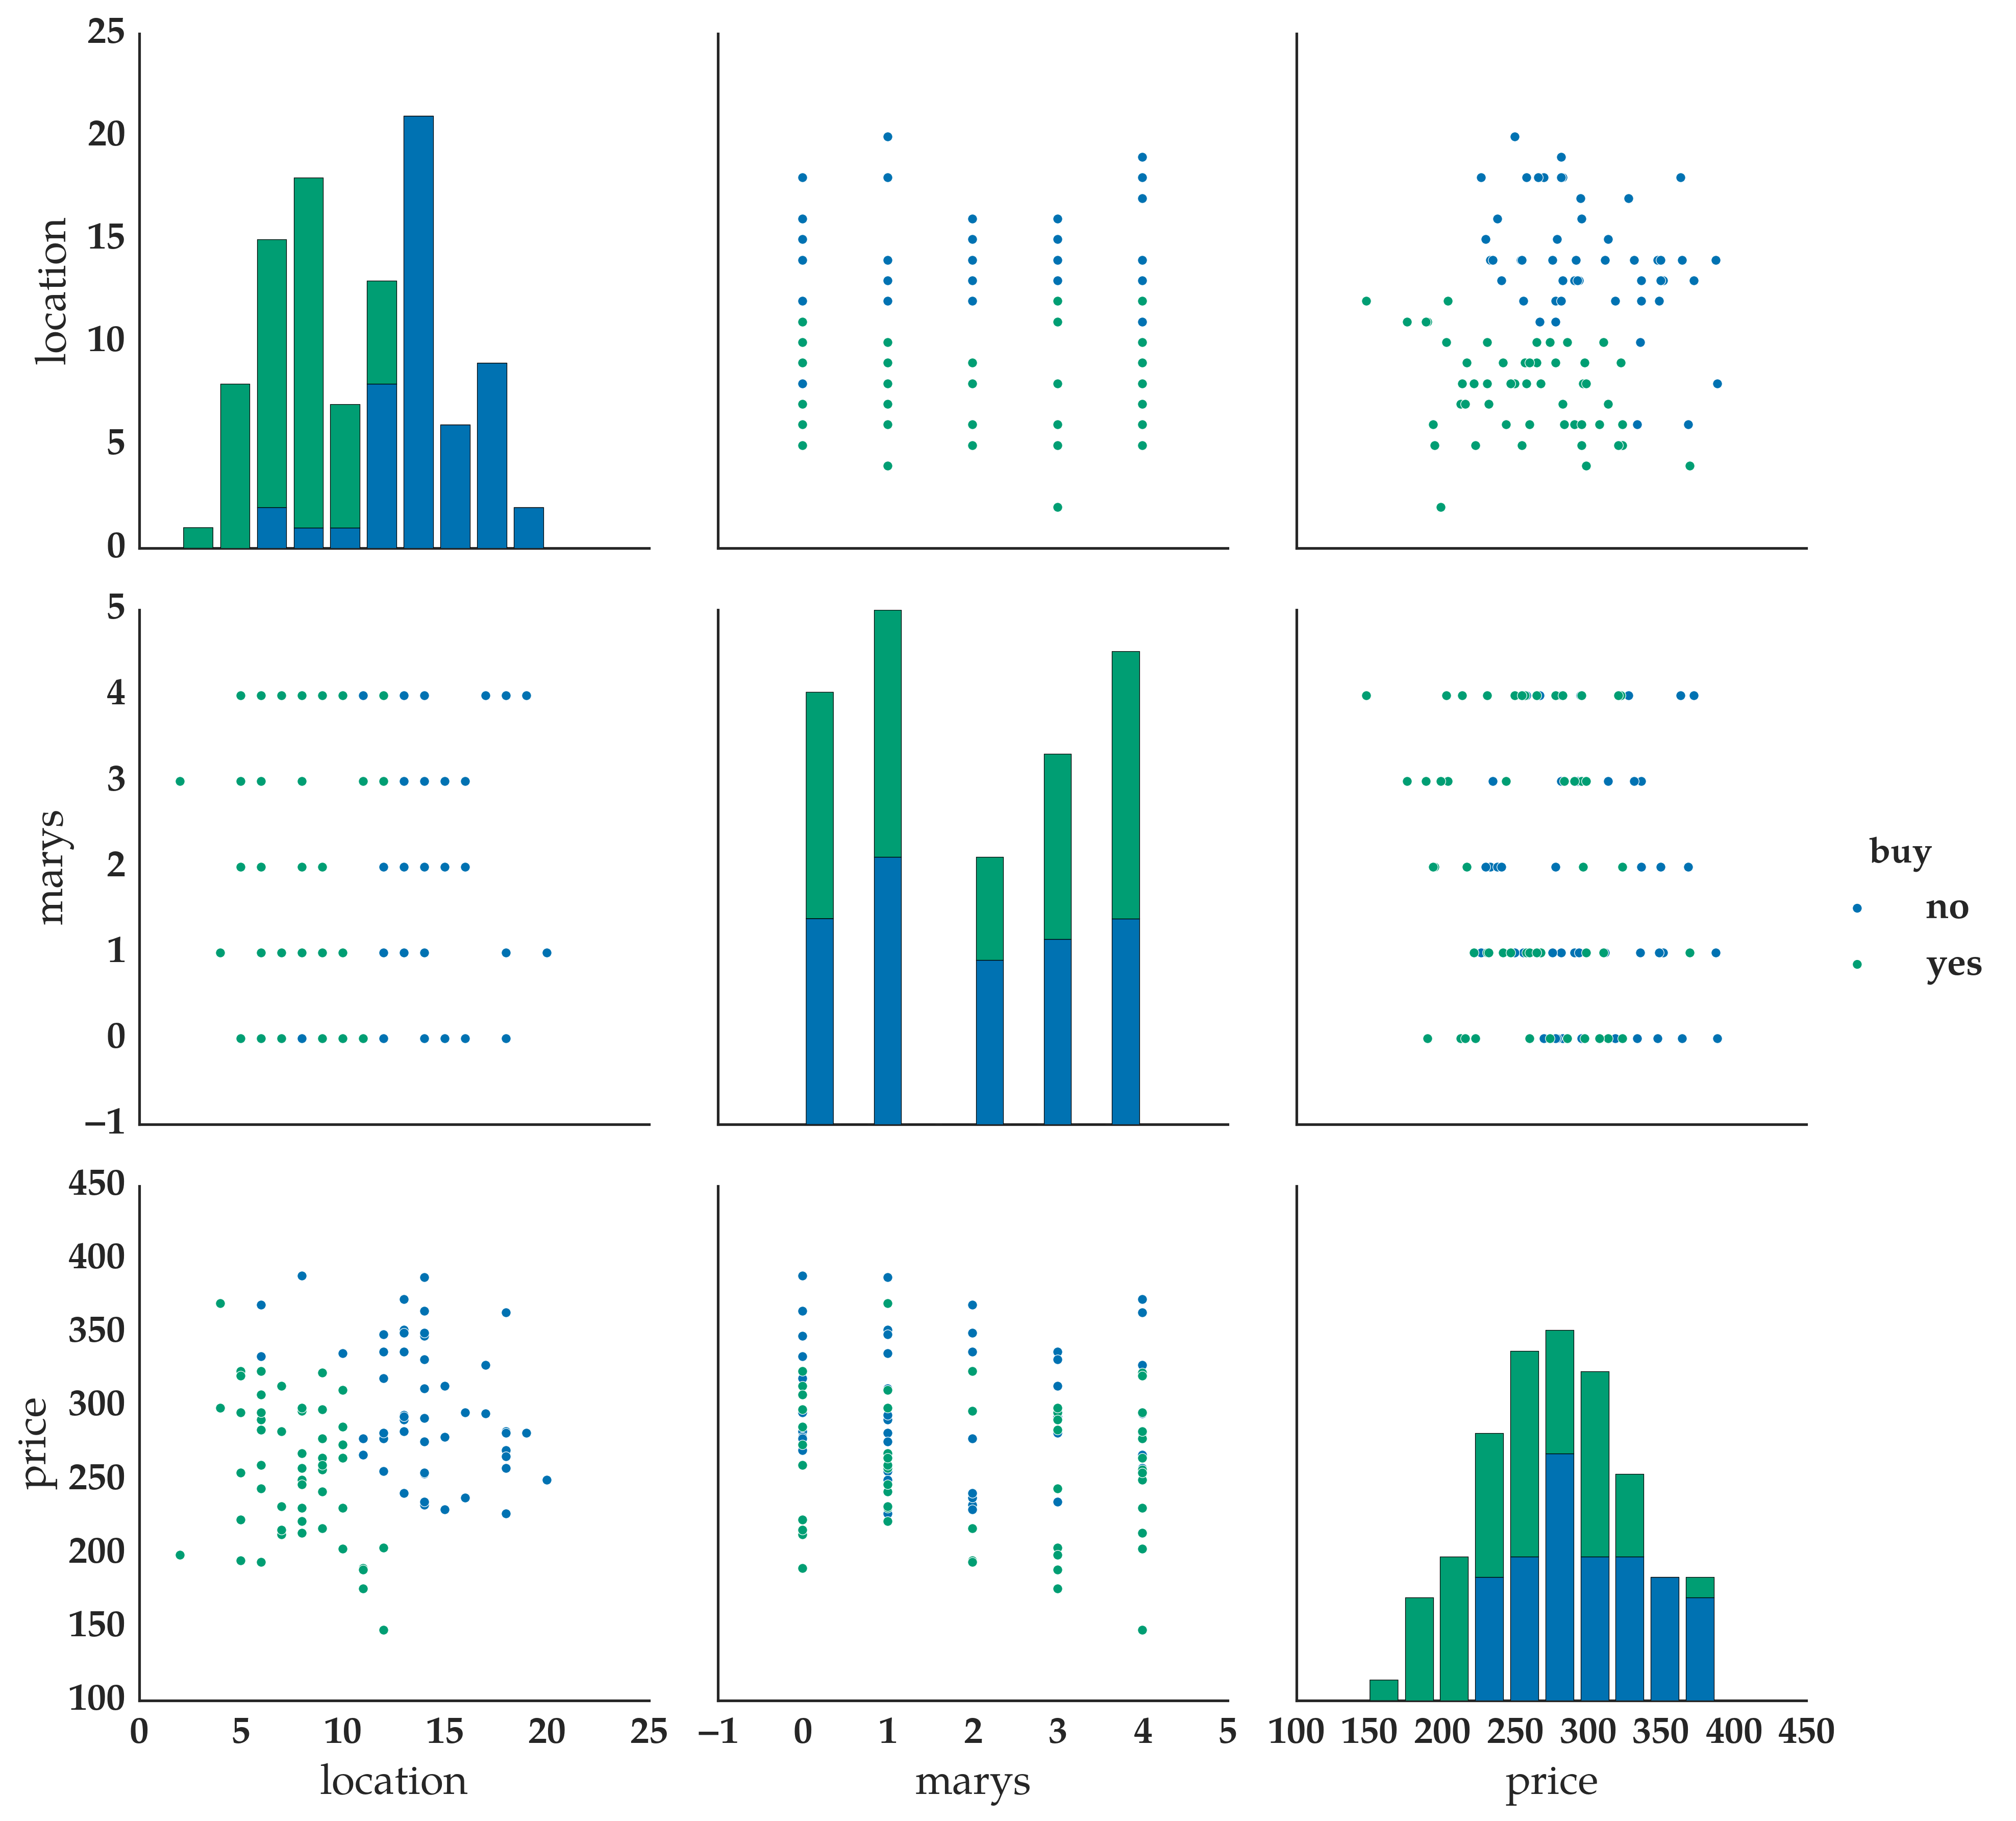
\includegraphics[scale=0.2]{figures/houses_grid.png}
    \end{column}
    \begin{column}{0.5\linewidth}
      \vspace{-0.6cm}
      \begin{center}
        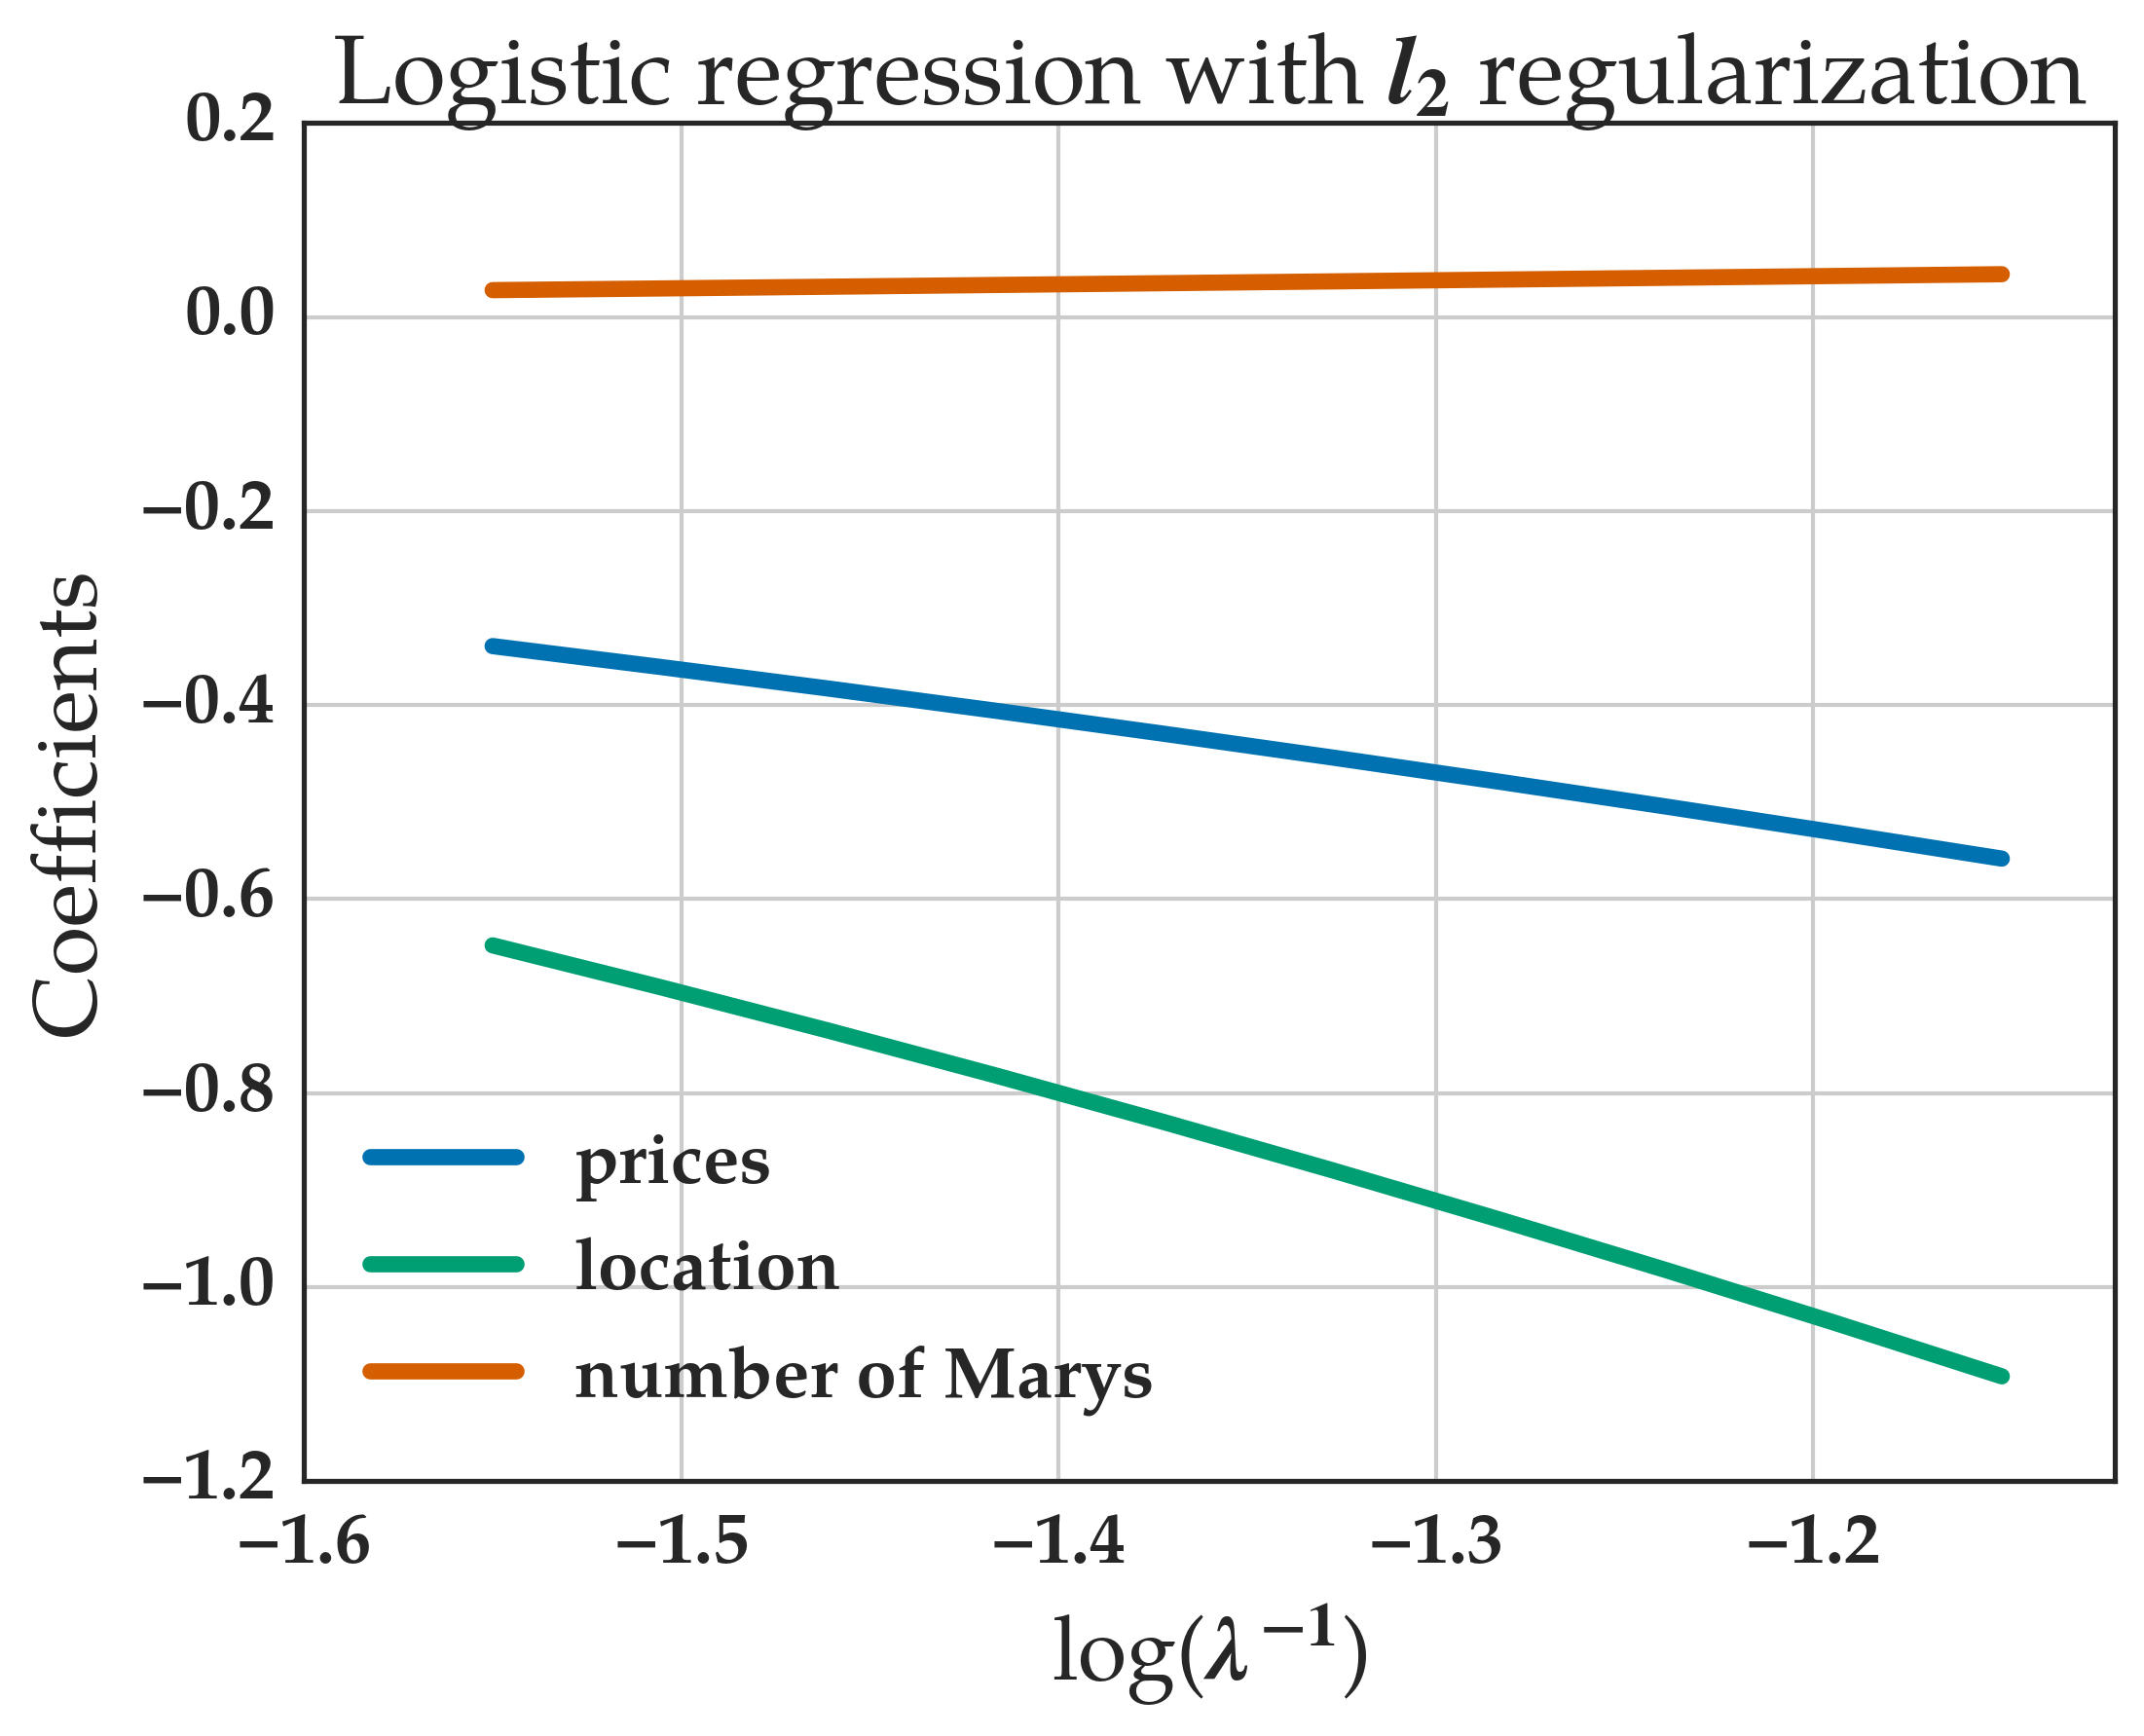
\includegraphics[scale=0.2]{figures/logistic_regression_l2_coef_path.png}
      \end{center}
      \begin{center}
        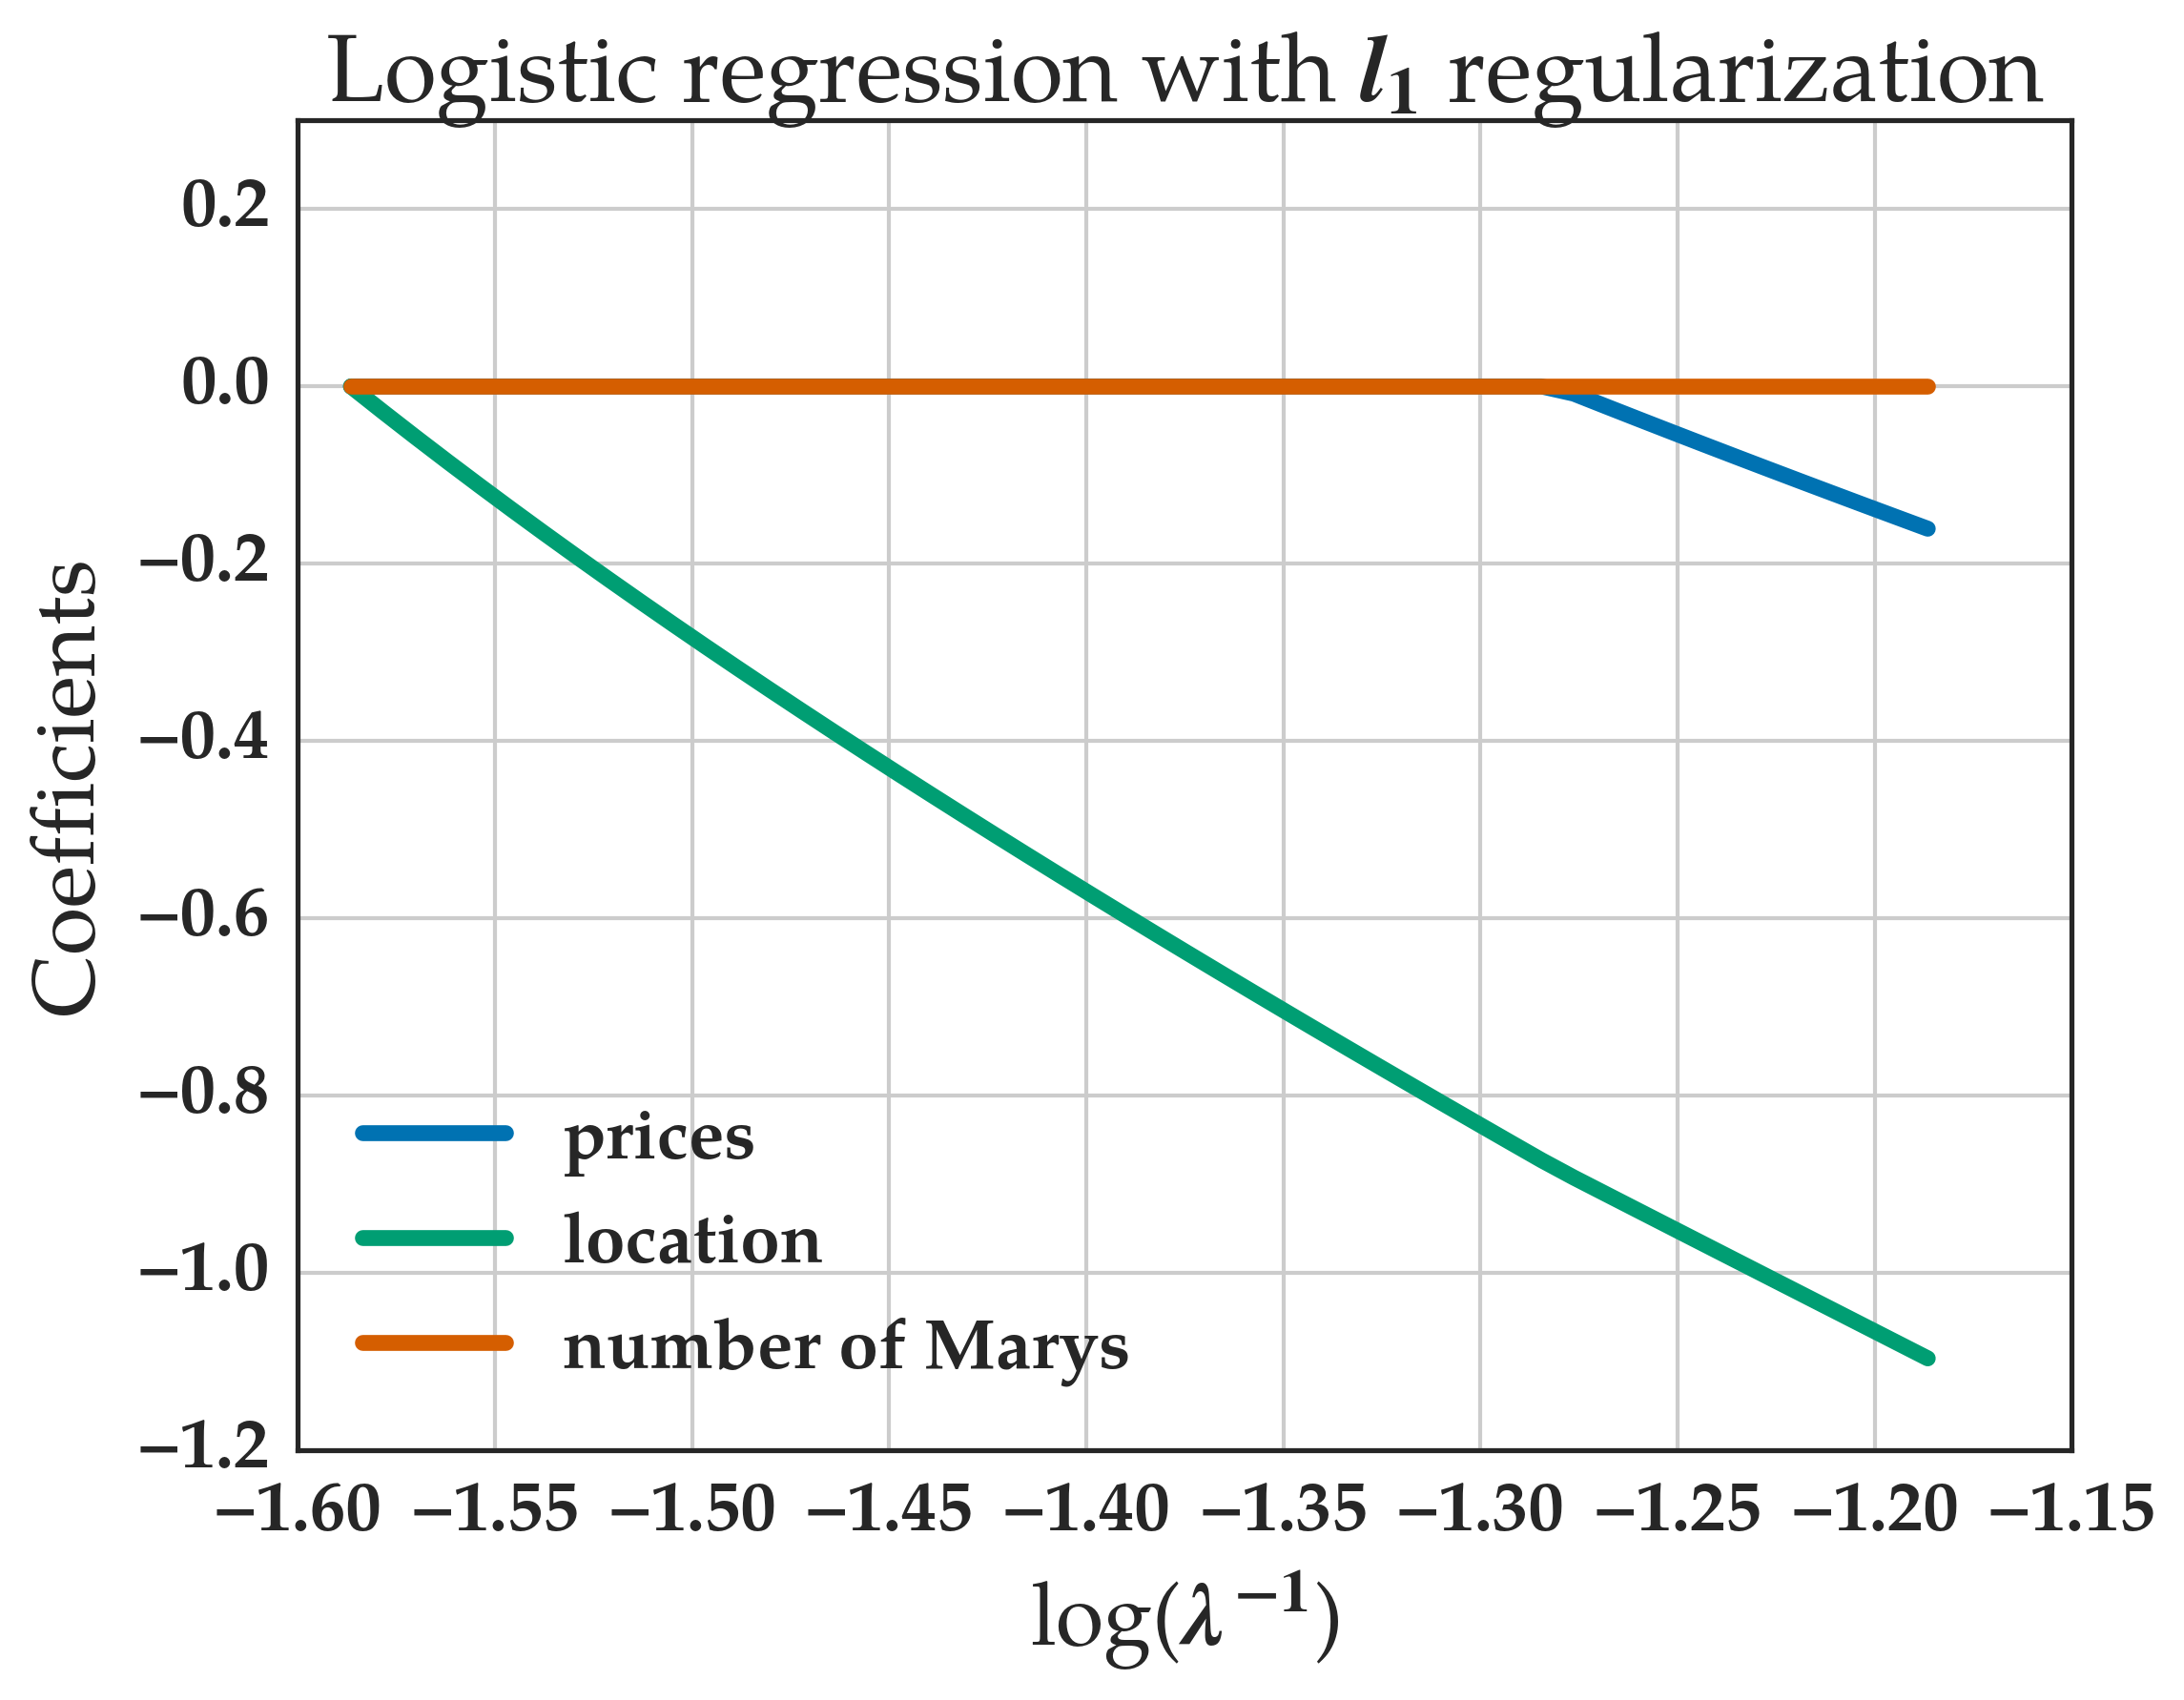
\includegraphics[scale=0.2]{figures/logistic_regression_l1_coef_path.png}
      \end{center}
    \end{column}
  \end{columns}
\end{frame}
\begin{frame}
  \frametitle{Regularization, Brain and Dimensionality}
  For fMRI decoding we no longer work with 2 or 3 dimensions. For
  whole brain analysis, the number of dimensions is very high (\(>10^{5}\)).

  An intuitive idea is that the space in which we work becomes \emph{emptier} as
  the number of dimensions gets larger, i.e., the input space is sparsely
  populated by the samples. 

  This is an ill-posed problem, thus we need regularization.

\end{frame}
\begin{frame}
  \frametitle{Curse of Dimensionality}
  \begin{center}
    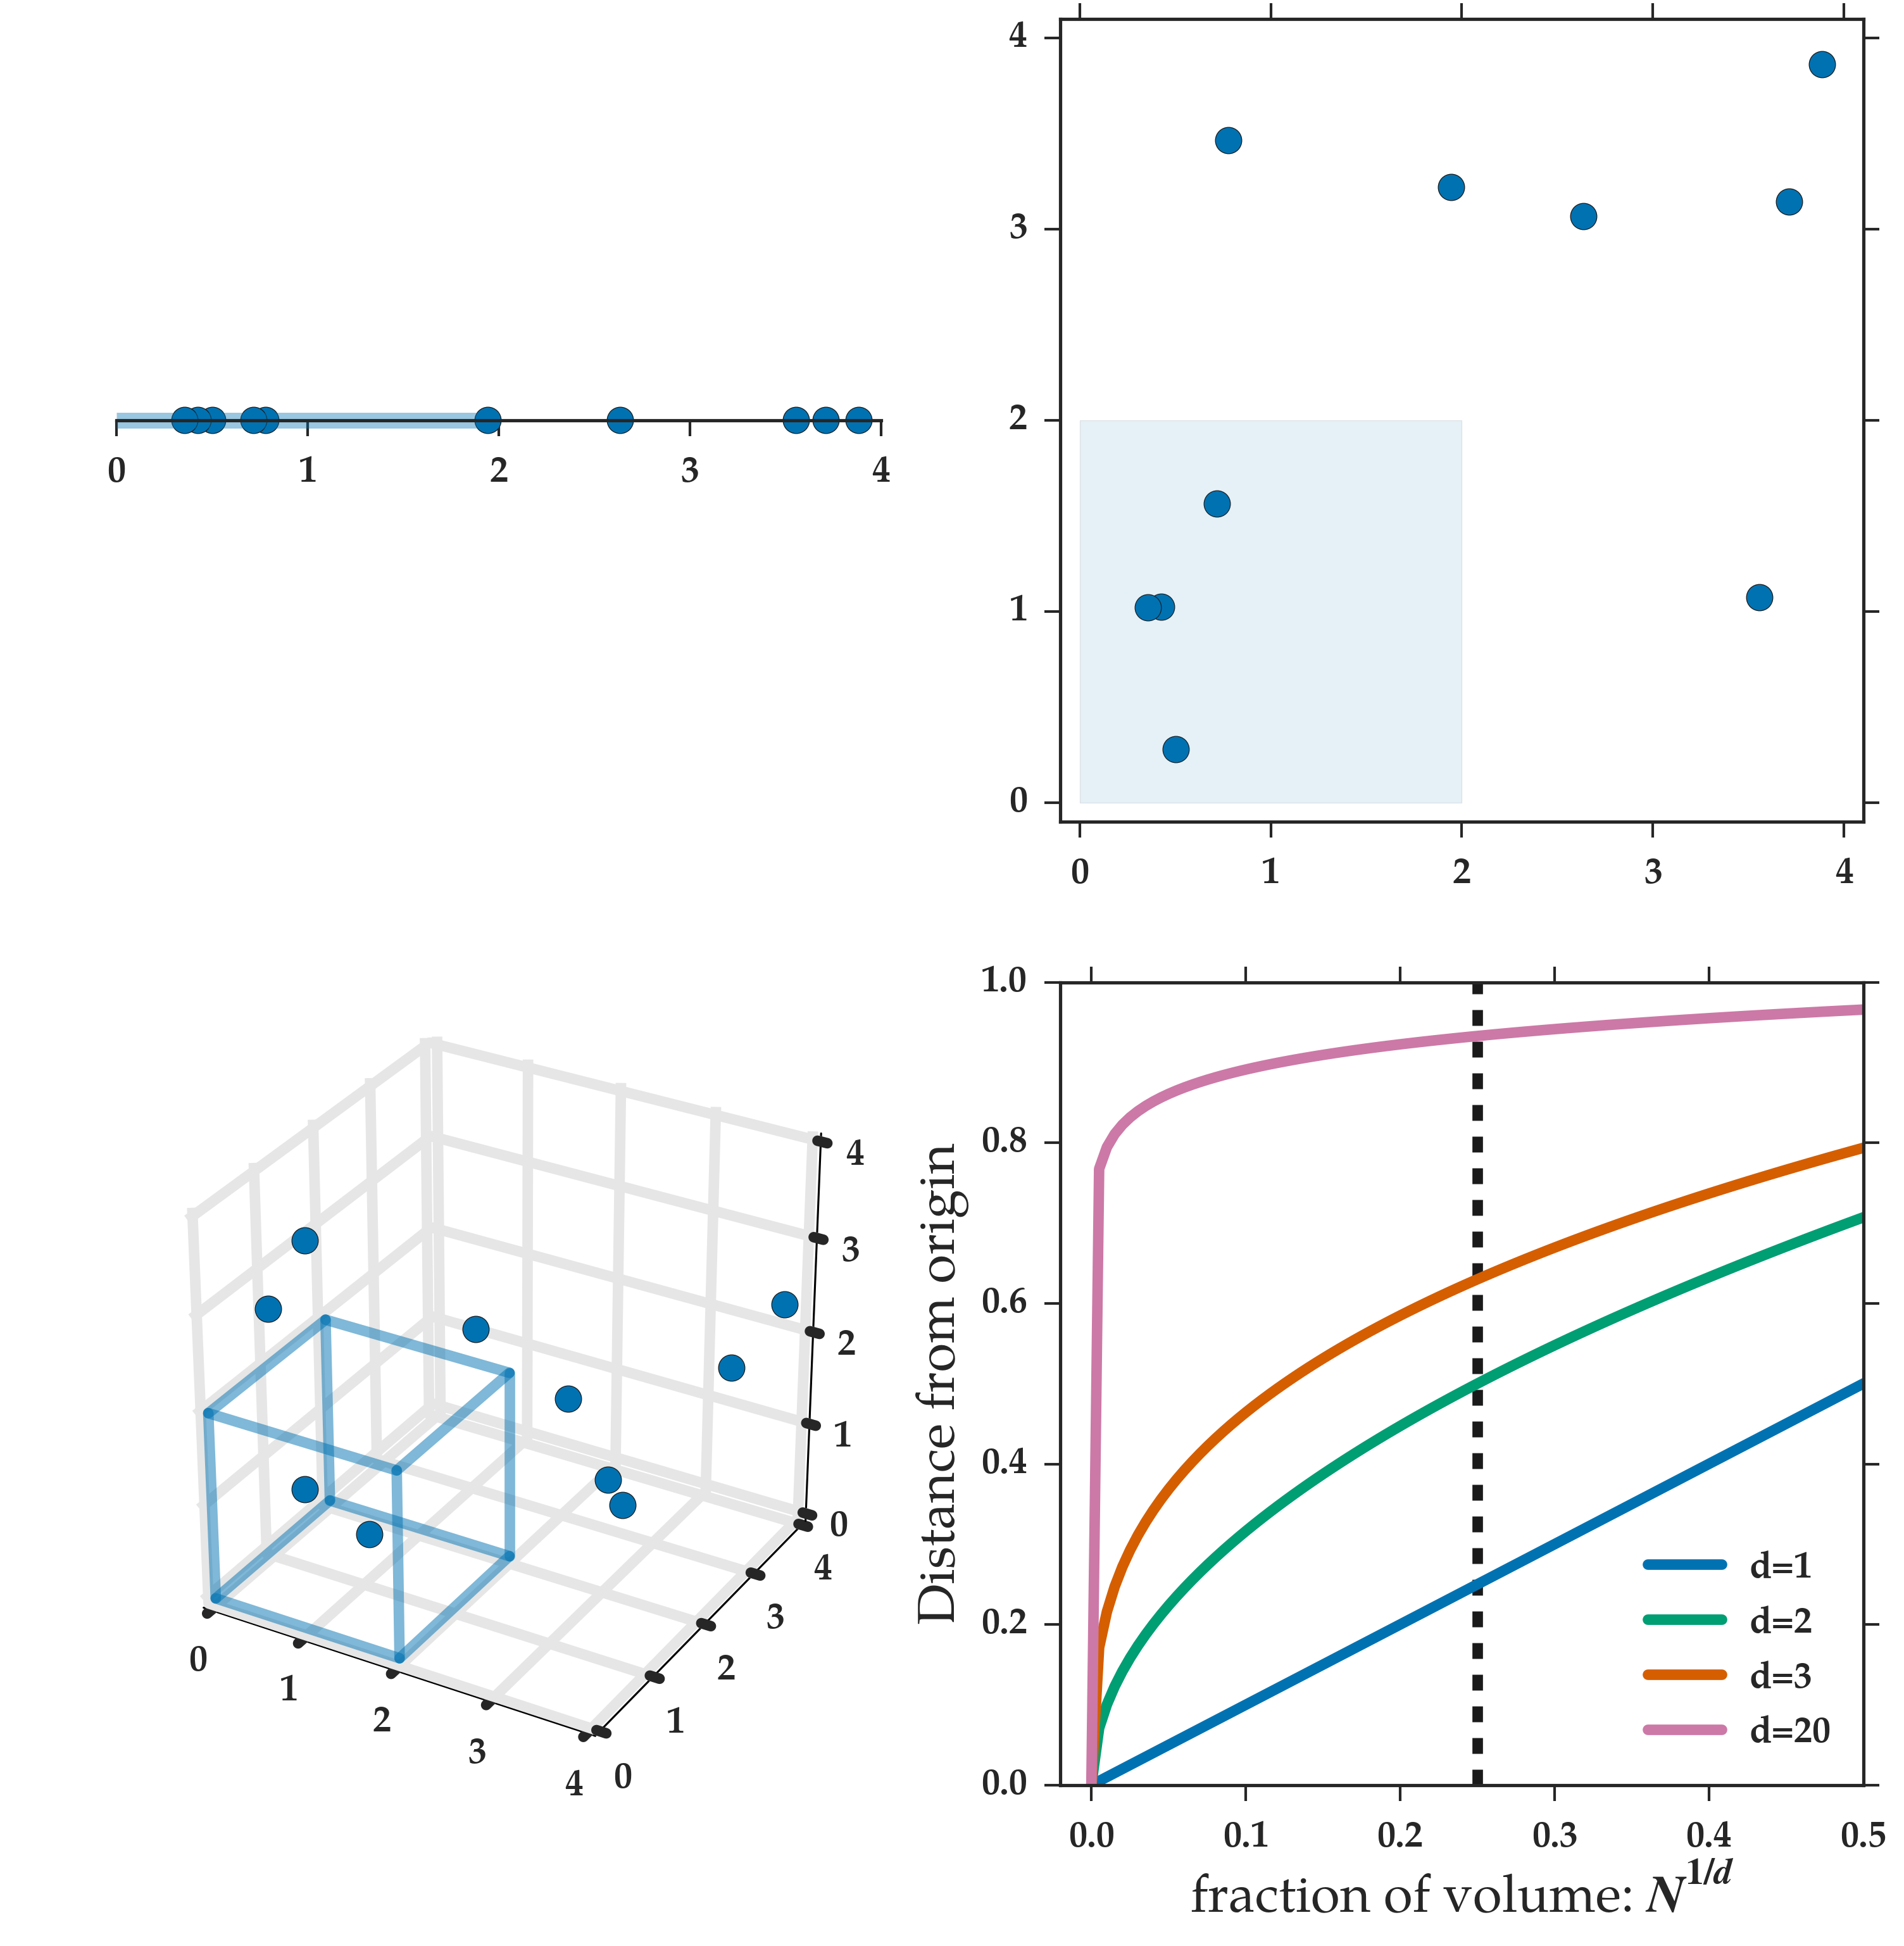
\includegraphics[scale=0.3]{figures/dimensionality.png}
  \end{center}
\end{frame}
% \begin{frame}
%   \frametitle{Structure}
%   We want to get sets of coefficients that allow interpretation of
%   psychophysical or psychological effects from particular tasks. But a brain has
%   a certain structure, this coefficients cannot appear anywhere.

%   Then, favor that neighbor voxels show consistent activation patterns. For
%   example, using anatomical priors.
% \end{frame}
\begin{frame}[t,shrink]
  \frametitle{Sparsity and Structure\footprnifullcite{baldassarre2012a}}
  From an experimental point of view, we expect to see increased activation in particular brain
  areas which corresponds to a sparse solution.
  
  However, a highly sparse model is prone to yield spatially incoherent activation
  patterns where features are picked up just to increase classification
  performance, ignoring others experimentally relevant.

  We can reduce the model sparsity with structural constraints, e.g. anatomical prior,
  to recover relevant features consistently.
\end{frame}
\begin{frame}
  \frametitle{Example: Instability in Sparse Models}
  An example of a highly sparse model: SVC with $l_1$ regularization and Haxby's
  faces vs. houses
    \begin{center}
      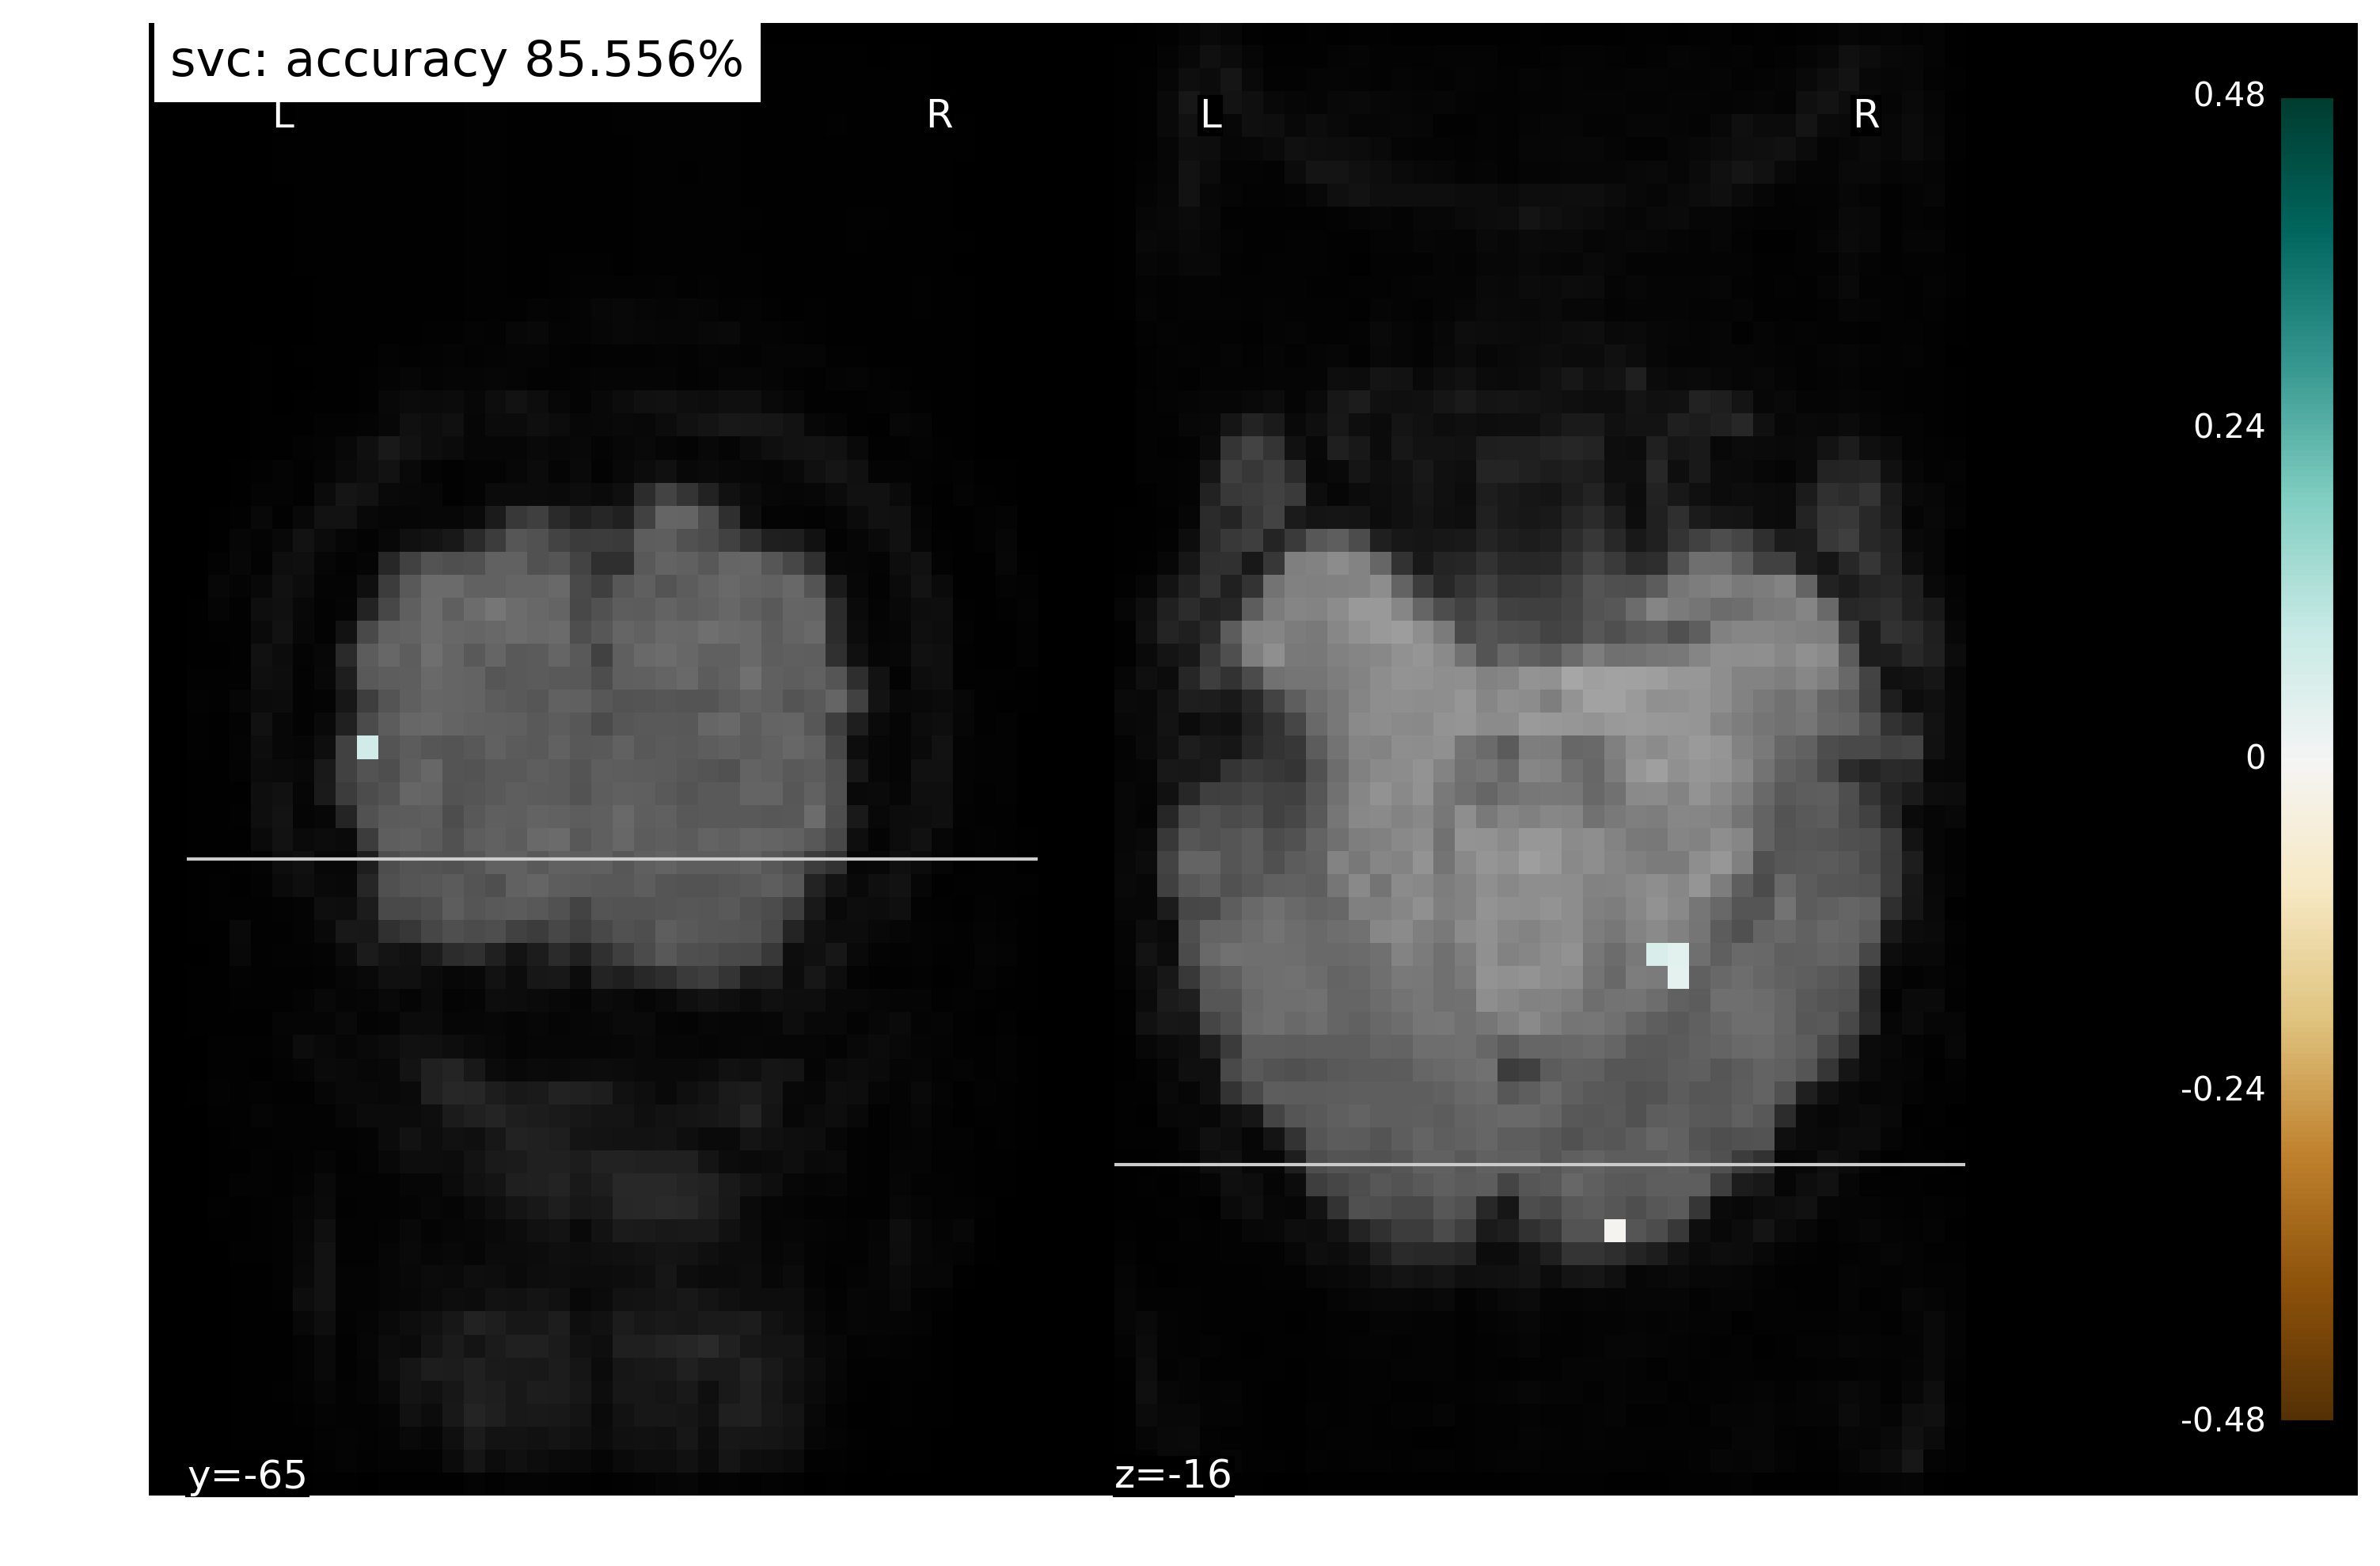
\includegraphics[scale=0.22]{figures/haxby_svc_plotmap_7e41.png}
      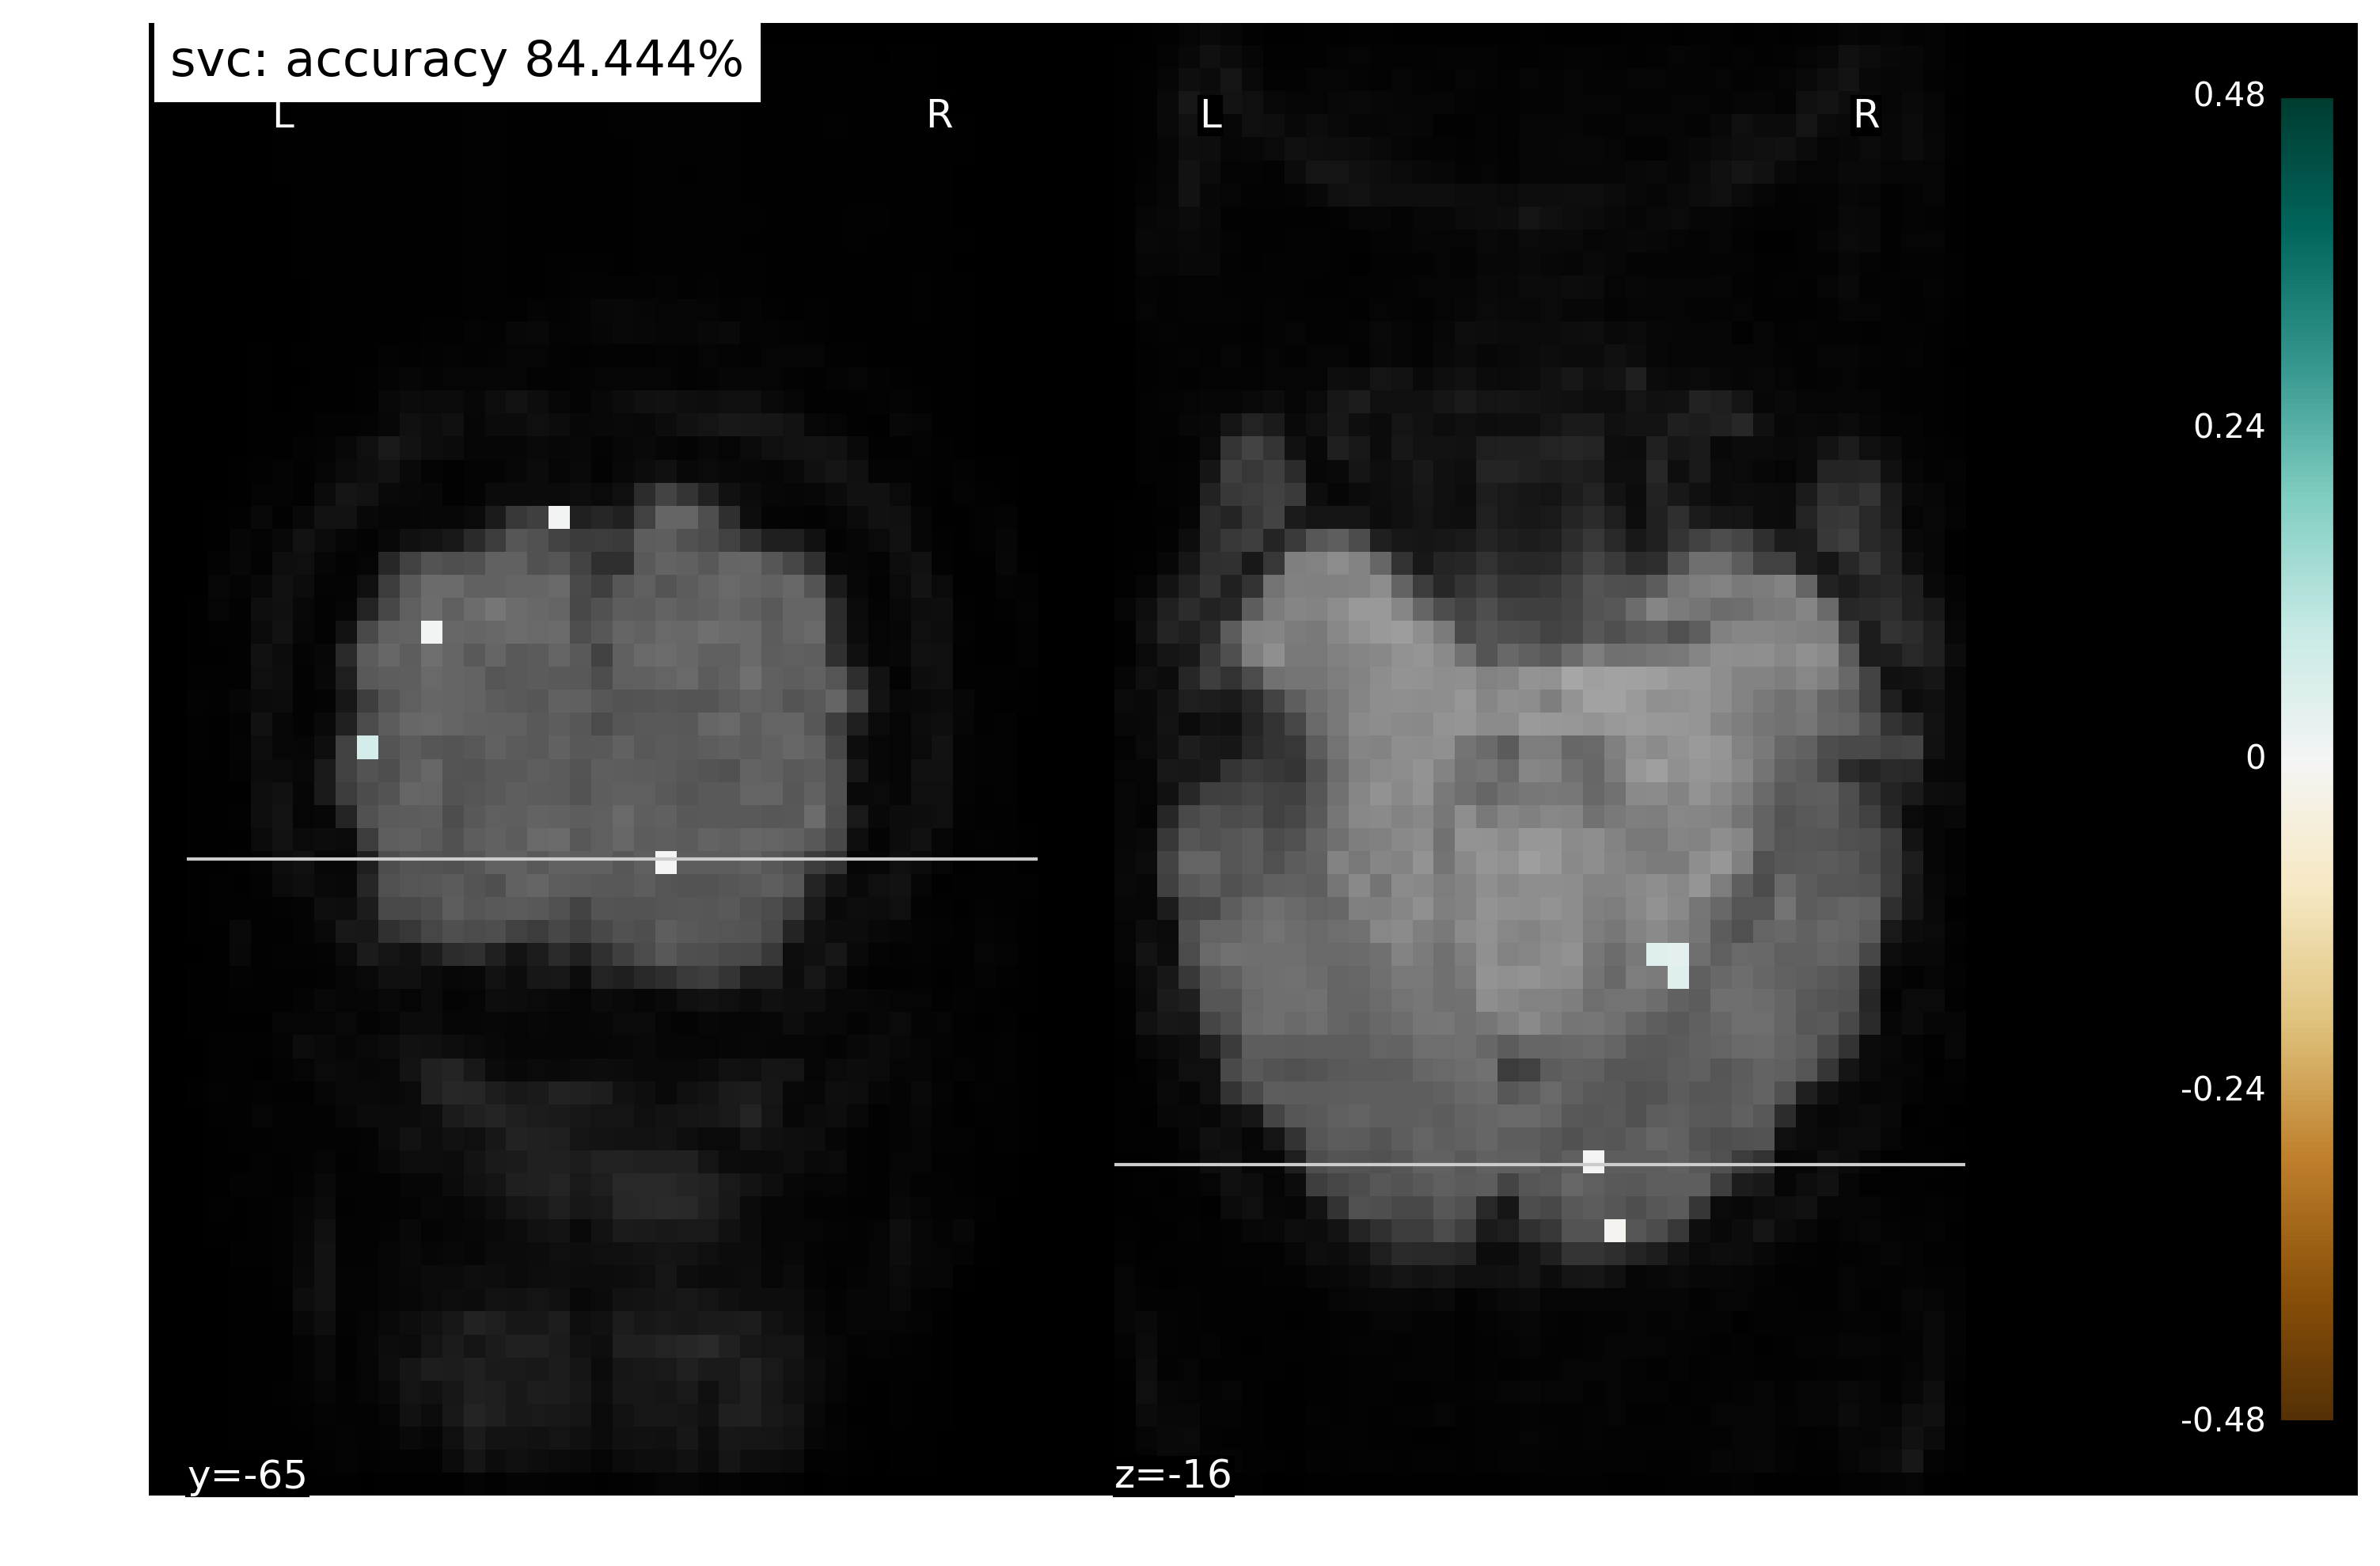
\includegraphics[scale=0.22]{figures/haxby_svc_plotmap_b073.png}
    \end{center}
    The outcome after running the same analysis with the same conditions: two
    different weight maps.
\end{frame}
\begin{frame}[t,shrink]
  \frametitle{Structured Sparsity: Graph-Net\footlessfullcite{grosenick2013}}
  Basic idea: look for a regularization term promoting sparsity and imposing
  structure at the same time.

  The starting point is the \emph{Elastic-Net}, a regression problem with
  \[J(\mathbf{w}) = \lambda_{1}\lVert{\mathbf{w}}\rVert_{1} + 
    \lambda_{2}\lVert{\mathbf{w}}\rVert_{2}^{2}\]

  where the \(l_{2}\) term is substituted by a new term
  \(\lambda_{G}\lVert{\mathbf{w}}\rVert_{G}^{2}\). The new term can incorporate
  spatial and temporal information, e.g. using the discrete Laplacian.

  Derivatives of the coefficients encourage smooth solutions
  (i.e., penalize roughness) while the $l_{1}$ term promotes sparse solutions. 

\end{frame}
\begin{frame}
  \frametitle{Structured Sparsity: TV-$l_1$\footprnifullcite{gramfort2013}}
  The idea behind \emph{Sparse Total Variation} (TV-$l_{1}$) is similar to
  Graph-Net. 

  \[J(\mathbf{w}) = \lambda \left( \lVert{\mathbf{w}}\rVert _{1} + 
   \lVert{\nabla\mathbf{w}}\rVert _{1}\right) \]

  This time, the TV term, $\lVert{\nabla\mathbf{w}}\rVert _{1}$ favors sharp
  contours and piece-wise constant solutions to the regression problem, in contrast
  with the Graph-Net that prefers smoother solutions.
\end{frame}
\begin{frame}[t]
  \frametitle{Example: Noisy Data}
  A set of simulated noisy data consisting of 30 samples and 2 clases. 
  \begin{center}
    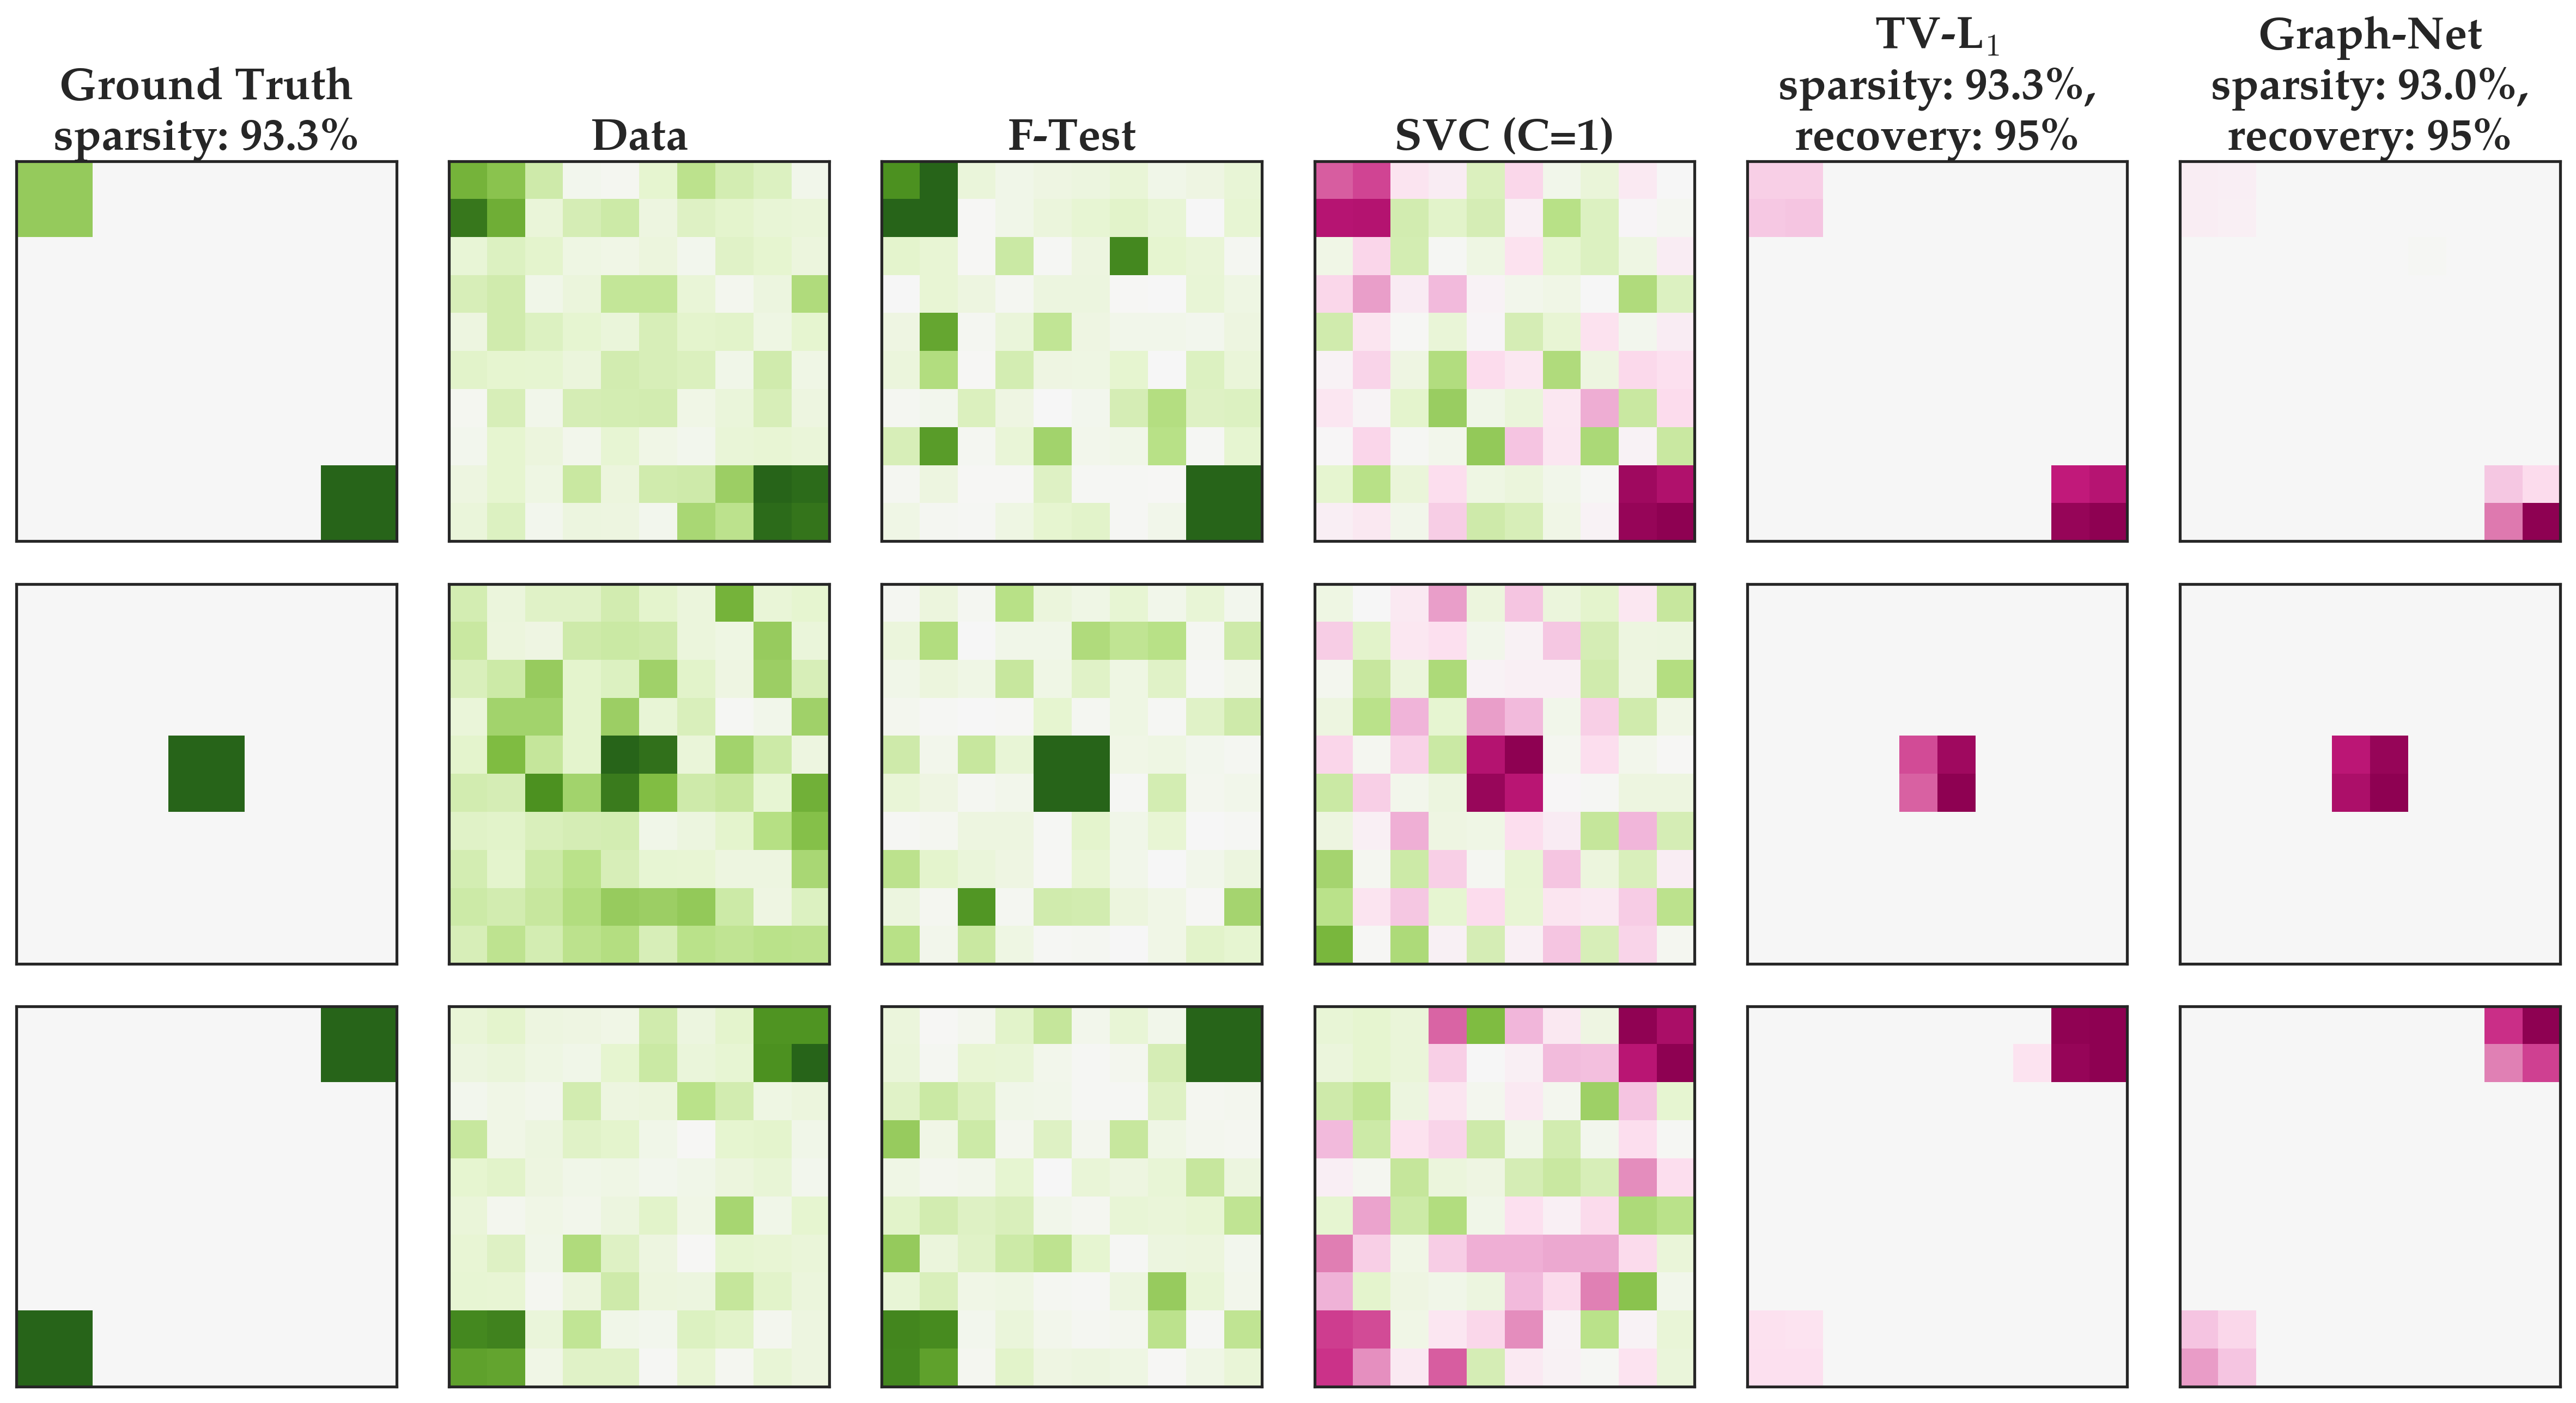
\includegraphics[scale=0.25]{figures/weights_synthetic_data_2.62_cbc.png} 
  \end{center}
\end{frame}
\begin{frame}[t]
  \frametitle{Example: Noisier Data}
  Same ground truth but noisier data.
  \begin{center}
    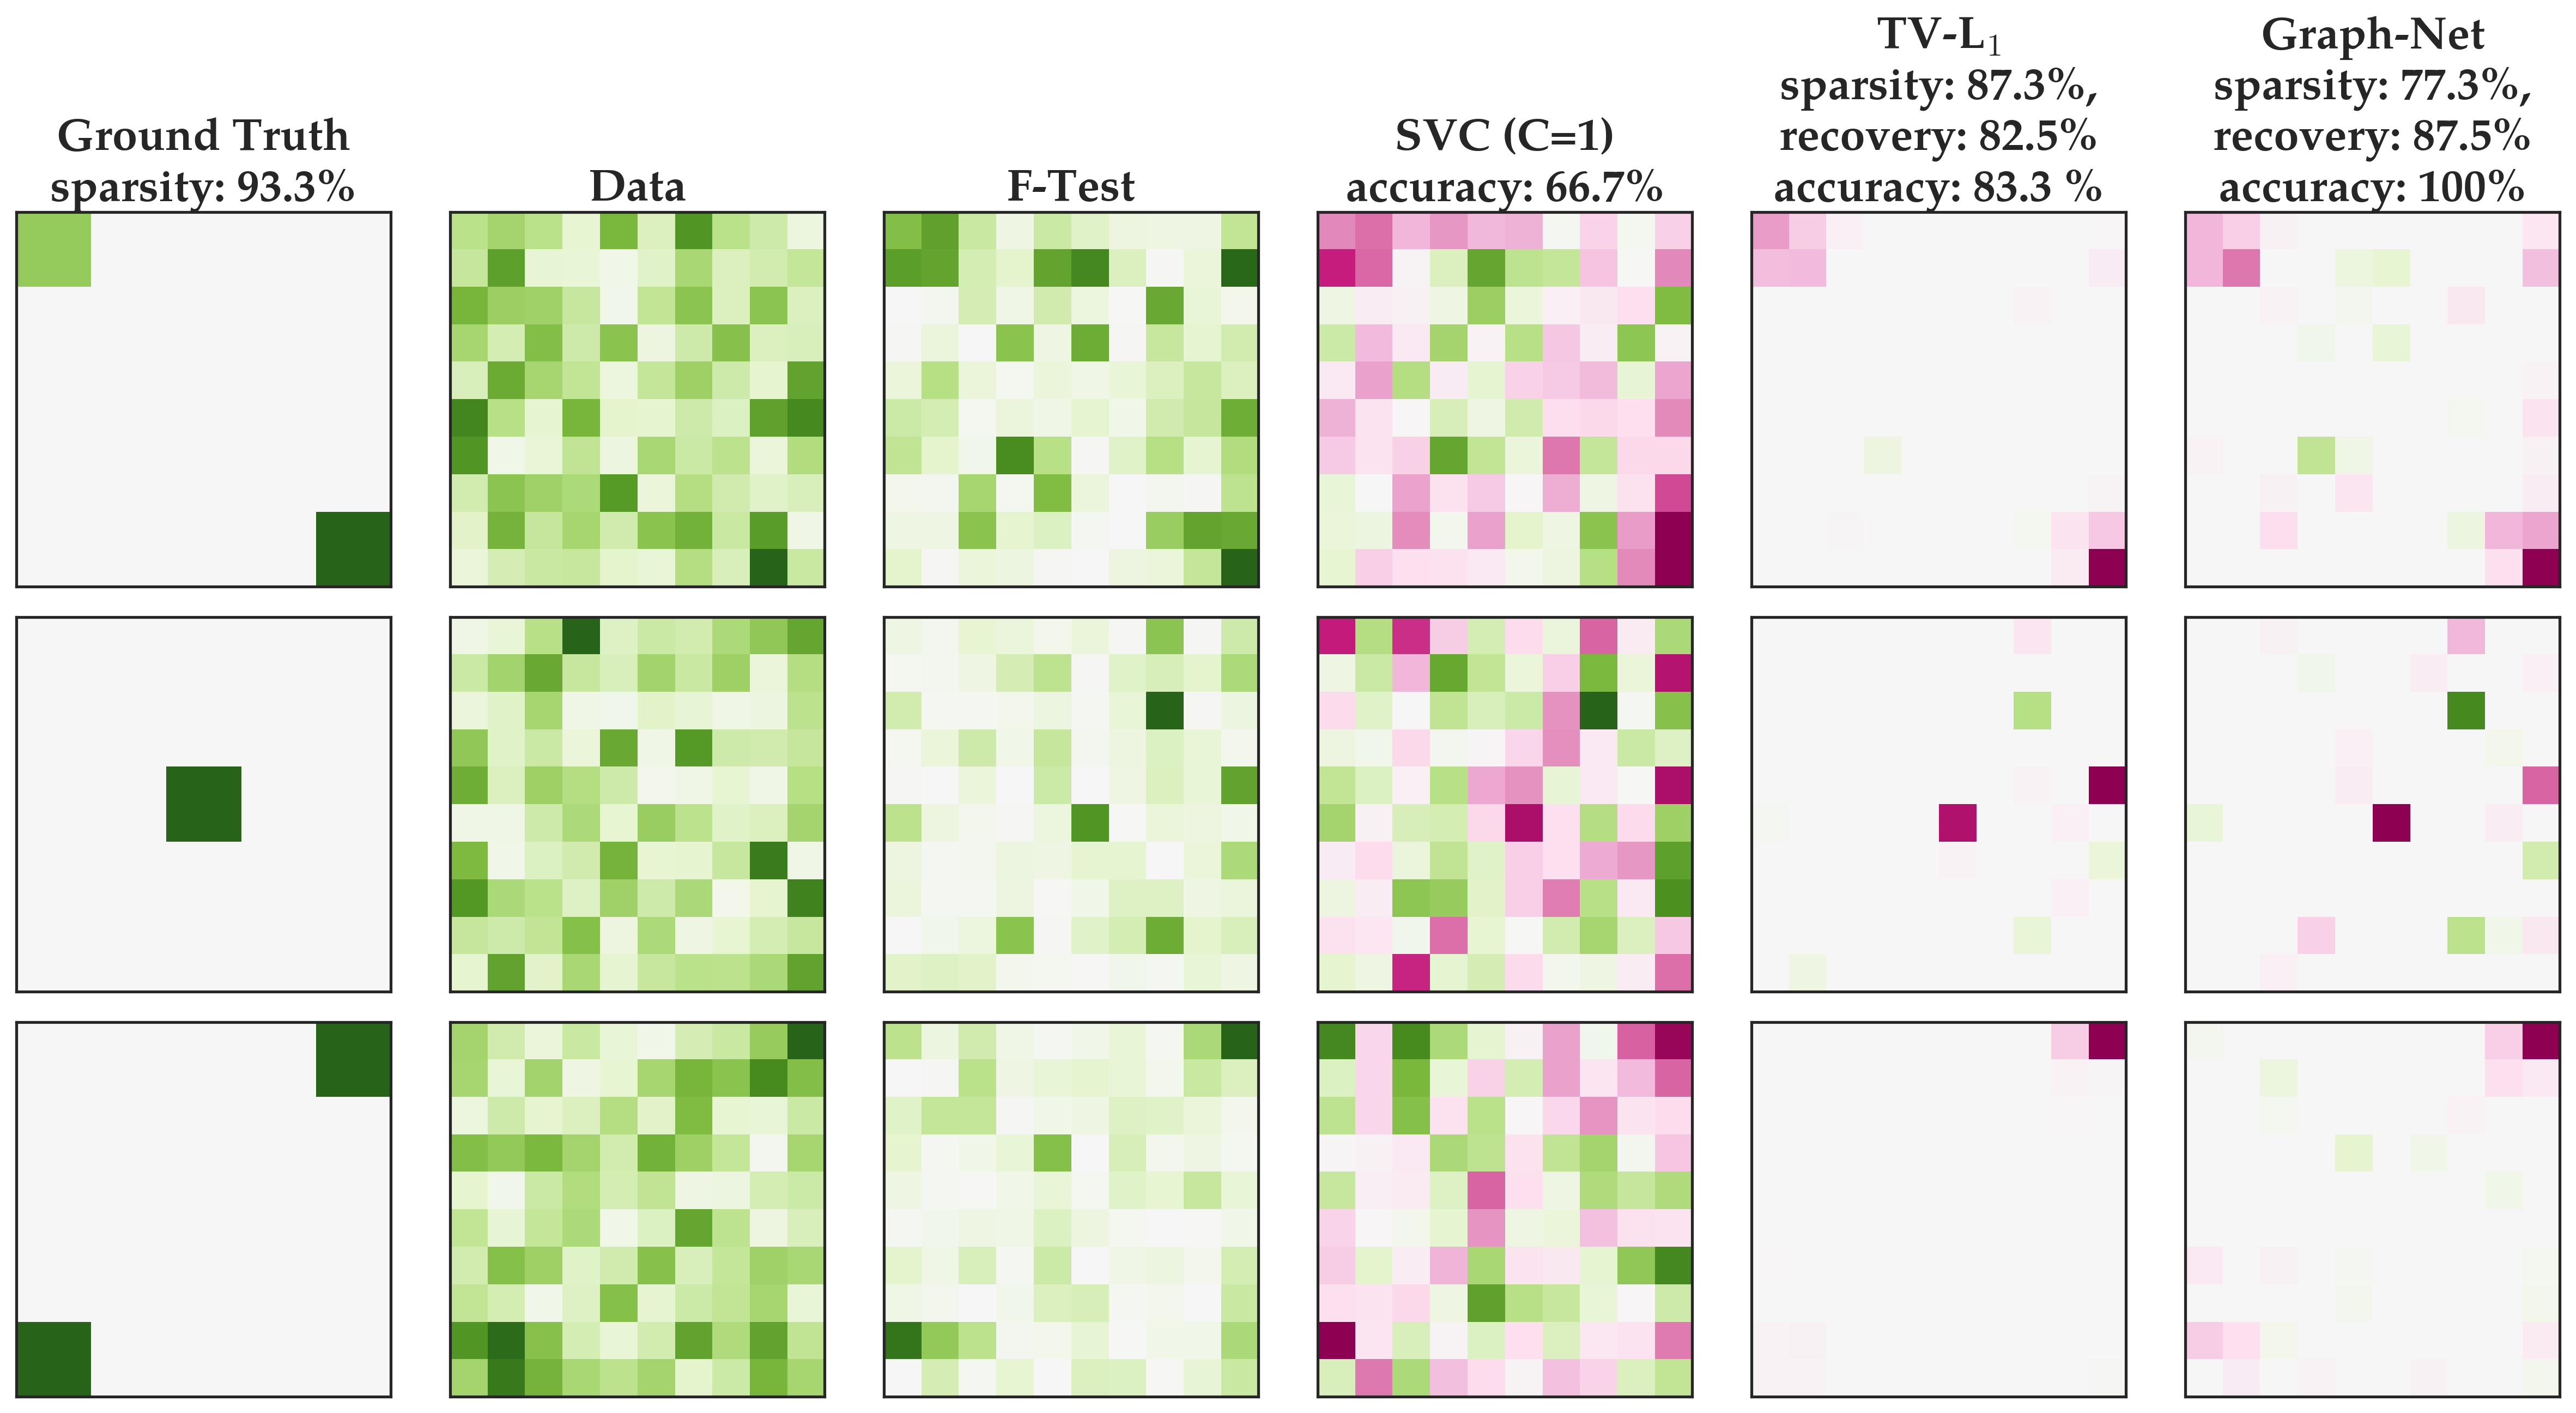
\includegraphics[scale=0.25]{figures/weights_sparse_synthetic_data_1.39_cbc.png} 
  \end{center}
\end{frame}
\begin{frame}[t,shrink]
  \frametitle{Conclusions/Remarks}
  % \fontsize{10pt}{8}\selectfont
  In summary, these methods can find balanced solutions between dense and very
  sparse models by being constrained by structural and/or temporal information used as
  priors.

  Structured sparsity offers
  \begin{itemize}
  \item interpretable results where coefficient maps are driven by data and
    not from classifier behavior,
  \item stable weight maps,
  \item a more adequate decoding method for neuroimage data.
  \end{itemize}

  But,
  \begin{itemize}
  \item there may be loss of accuracy in favor of increase in recovery: helps
    interpretation,
  \item the parameter space needs to be optimized,
  \item and can be slower than other methods.
  \end{itemize}
\end{frame}
\begin{frame}
  \frametitle{Software}
  Implementations to try:
  \begin{itemize}
  \item nilearn (not officially released) \\
\texttt{nilearn.github.io}

\item neuroparser \\
\texttt{github.com/logang/neuroparser}
  \end{itemize}
\end{frame}
\begin{frame}[standout]
    Thank you! \\
    Questions?
\end{frame}

%% -- backup slides --
%% backup slides go after appendix as normal frames. See theme documentation
%% and include \usepackage{appendixnumberbeamer} so that they do not count
%% towards the total number of slides in the main presentation
\appendix
\begin{frame}{Appendix}
    SpaRSA implementation
\end{frame}
\begin{frame}{Taks fMRI Decoding}
    Predict the behavioral task, i.e. category or class.
\end{frame}
\end{document}
% Local Variables:
% TeX-engine: xetex
% coding: utf-8
% mode: latex
% TeX-master: t
% TeX-command-extra-options: "-shell-escape"
% End:
